
%% Empiezo en capítulo 0.
\setcounter{chapter}{-1}

%% Para no mostrar el "Capítulo N" antes del título del capítulo:
\titleformat{\chapter}[display]{\normalfont\bfseries}{}{0pt}{\Large}
\titlespacing*{\chapter}{0pt}{10pt}{20pt}

\chapter[Hoja de Identificación]{
    \thispagestyle{empty}
    \normalsize
    \mdseries
    \Huge\bf{Hoja de Identificación}
}

\pagenumbering{arabic}
\setcounter{page}{1}
\begin{itemize}
    \item \textbf{Título del proyecto:} Sistema de avisos para discapacitados auditivos \\
    \item \textbf{Código del proyecto:} 000001 \\
    \item \textbf{Datos del cliente:} \\
        \begin{itemize}
            \vspace{-0.4cm}
            \item Universidad de Cádiz (Escuela Superior de Ingeniería)
            \item Avenida de la Universidad de Cádiz Nº10, 11519 Puerto Real
            \item 956 48 32 00
            \item direccion.esi@uca.es
        \end{itemize}
    \item \textbf{Datos del suministrador:} \\
        \begin{itemize}
            \vspace{-0.4cm}
            \item Raúl Díez Sánchez
            \item Ingeniero Informático
            \item Calle Sagasta Nº 56 1ºA, 11002 Cádiz
            \item 653 50 41 47
            \item ra.diezsanchez@alum.uca.es
        \end{itemize}
\end{itemize}

\vspace{2cm}

Firmado:

\vspace{-0.9cm} 
\begin{flushright} Cádiz, \today \end{flushright}

\vspace{2cm}

\begin{table}[h]
    \centering
    \begin{tabular}{lr}
        Raúl Díez Sánchez & \hspace{9cm}Cliente
    \end{tabular}
\end{table}
\newpage


%% Cambio de nuevo el formato del título, ahora en lugar de
%% "Capítulo N" es "N. TÍTULO_DEL_CAPÍTULO"
\titleformat{\chapter}{}{}{0em}{\bf\Huge\thechapter.~}

\chapter{Introducción}
Cada día más, la tecnología nos muestra lo útil que puede llegar a ser para simplificar o ayudar en nuestro día a día. Un ejemplo de esto son la domótica y los proyectos AAL (o de vida asistida en la vivienda, por sus siglas en inglés) que surgen a raíz de la domotización. \\

La tecnología ayuda a solventar grandes necesidades, con soluciones cada vez mejores y más adaptadas. La accesibilidad es una de las grandes necesidades de la sociedad: permitir que un producto o servicio pueda ser utilizado por todos los posibles usuarios, incluyendo personas con diferentes capacidades o discapacidades. \\

Existen diversas discapacidades, y todas presentan un gran problema a la hora de que las personas que las padecen sean autónomas. Una de estas discapacidades es la auditiva. El simple hecho de estar en casa puede ser un gran problema, como lo es no saber cuándo llaman a la puerta.

\chapter{Objetivo}
El objetivo de este proyecto es crear un sistema para adaptar la vivienda de una persona o personas con discapacidad auditiva, de manera que puedan determinar en todo momento si alguien del exterior está intentando comunicarse con alguien en el interior de la vivienda. \\

Se pretende implantar un sistema de avisos visuales, que el discapacitado pueda ver, comprender y actuar conforme a la alerta.

\chapter{Antecedentes}
Actualmente existen varias soluciones a los problemas que pueda tener una persona con discapacidad auditiva, independientes del grado de discapacidad que padezca.\\
\\
Una de las soluciones consiste en un aparato de bolsillo de avisos por señales de vibración y luces de colores~\cite{visiofarma}, que recibe los avisos de distintos aparatos receptores de ruido que pueden obtener información del ruido generado por el timbre, el teléfono, el portero automático...\\
\\
Esta solución requeriría que el discapacitado lleve consigo siempre un aparato en el bolsillo, lo cual puede ser un poco molesto. Además, tiene una limitación de número de alarmas a captar.\\
\\
Otra posible solución es la instalación de ventanas en la mayoría de las paredes de la vivienda (paredes interiores), que permitiría ver las alertas visuales desde cualquier habitación. Este sistema necesitaría que previamente se modificasen los aparatos que emiten alertas sonoras para que emitan alertas visuales, además de reducir la intimidad de las personas que habiten en la vivienda.\\
\\
Una solución diferente a las anteriores es adaptar la instalación eléctrica de la vivienda~\cite{avisossordos}, instalando tantas lámparas por habitación como alertas visuales se quieran mostrar. Estas lámparas mostrarían alertas visuales para el teléfono, el timbre, etc. La mayor desventaja aquí es el consumo de bombillas necesarias para una instalación completa, y el espacio que estas ocuparían.

\chapter{Descripción de la Situación Actual}
Hoy día, en cualquier vivienda existen demasiadas alertas sonoras como para controlarlas todas. Se pretende así por tanto tratar las alertas más importantes para que las personas con discapacidad puedan percibir los avisos más importantes.

\section{Informe de diagnóstico}
\label{sec:informediagnostico}

En este punto se tratan los distintos aspectos a tener en cuenta dentro de una vivienda estándar en cuanto a alertas se refiere. Este informe es la base de parte de los requisitos no funcionales.

    \subsection{Timbre de la puerta}

    Un caso es el timbre de la puerta, donde una persona con discapacidad auditiva es poco probable que sea capaz de percibir las alertas que genere.

    \subsection{Telefonillo (portero automático)}

    Otro caso es el del portero automático, del cual existen 2 tipos básicos: analógicos y digitales. Pese a que los telefonillos digitales son tecnológicamente superiores, se siguen utilizando telefonillos analógicos, debido a su bajo coste en comparación. Además, históricamente, el uso del telefonillo analógico es más extendido. Debido a estas razones, en este Proyecto se tendrá en cuenta el uso de telefonillo analógico, para abarcar un mayor rango de posibles instalaciones.

    Entre los telefonillos analógicos, existen 2 tipos atendiendo al tipo de llamada que realizan:
    \begin{itemize}
        \item Llamada zumbador.
        \item Llamada electrónica.
    \end{itemize}

    La diferencia principal entre ambos reside en su funcionamiento y la forma de generar la alerta sonora~\cite{llamadatelefonillo}.

    \begin{itemize}
        \item \textbf{Telefonillos analógicos de llamada zumbador}: En los telefonillos con llamada zumbador, una vez que se realiza la llamada, el grupo fónico de la placa exterior a la vivienda genera una señal alterna de 12 Vac que envía por el hilo de llamada. La señal alterna llega al zumbador situado en el teléfono, haciendo que el zumbador vibre y finalmente produzca el sonido de la llamada.
        \item \textbf{Telefonillos analógicos de llamada electrónica}: En los telefonillos con llamada electrónica, una vez que se realiza la llamada, el grupo fónico de la placa exterior a la vivienda genera una señal formada por diferentes frecuencias, y la envía por el hilo de llamada. La señal llega al altavoz del auricular del teléfono, produciendo el sonido de la llamada. La llamada puede ser de varios tipos en función del número de frecuencias utilizadas.
    \end{itemize}

    Teniendo en cuenta que los de llamada zumbador envían una señal de 12 Vac, y los de llamada electrónica una señal de varias frecuencias, es más fácil trabajar con los del primer tipo, pudiendo darse soluciones electrónicas bastante sencillas. Además, son el tipo más extendido, y el que más probabilidades hay de encontrar en una vivienda. Se utilizará por tanto un telefonillo de este tipo para la implementación del sistema y la demostración de funcionamiento.

    \subsection{Bombillas}

    En cuanto a las bombillas existentes en una vivienda, las más empleadas son las bombillas de casquillo E27, también llamadas bombillas de rosca Edison. Por tanto, para abarcar un mayor rango de posibles instalaciones, este Proyecto se basará en el uso de bombillas de este tipo. \\

    En caso de manipular estas bombillas, existen dos posibilidades: hacerlo mediante la propia instalación eléctrica, o manipularlas de manera inalámbrica.

    \subsection{Router integrado}
    \label{sec:routerintegrado}

    Dentro de una vivienda habitualmente se puede encontrar un router integrado, dispositivo que integra las funciones y conexiones de un router, un punto de acceso WiFi y un switch Ethernet. Este dispositivo suele ser instalado por el Proveedor de Servicio de Internet (ISP) o incluso hay usuarios que adquieren un router integrado neutro (no ligado a un ISP) por separado.

\chapter{Normas y Referencias}
\section{Disposiciones legales y Normas aplicadas}

\begin{itemize}
    \item \textbf{UNE 157801:2007} - Criterios generales para la elaboración de proyectos de sistemas de información.
    \item \textbf{UNE 157001:2014} - Criterios generales para la elaboración formal de los documentos que constituyen un proyecto técnico.
\end{itemize}

    
%% Bibliografía como section.
\nocite{*}
\bibliographystyle{plain}
\bibliography{main}

\section{Metodología de desarrollo}

En este Proyecto se ha decidido optar por aplicar lo que se conocen como metodologías ágiles, siendo este tipo de metodologías las que se basan en la división del trabajo en determinadas secciones funcionales o etapas que se van revisando e incrementando, con el objetivo de detectar errores y corregirlos poco a poco, llegando a una solución del Proyecto más rápidamente que con las metodologías de desarrollo clásicas. \\

Dentro de las metodologías ágiles se ha decidido utilizar la denominada SCRUM, metodología que permite seguir un proceso incremental basado en la división y el desarrollo de funcionalidades que se validan y corrigen conforme se avanza en la realización del Proyecto. \\

Esto proporciona cierta flexibilidad en el desarrollo frente a cualquier tipo de cambio, ya que se pueden tratar como cambios menores. Si se compara esta con otro tipo de metodología, se puede apreciar que es una gran ventaja, ya que en otras metodologías en las que hay que desarrollar una versión de prototipo o una versión totalmente operativa a partir de la cual se corregirá lo que sea necesario, cualquier modificación puede suponer un sobre-coste o un gasto de tiempo con el que al seguir la metodología SCRUM se ahorra. \\

Otra gran ventaja de esta metodología es que el resultado suele ser de mayor calidad, ya que al abordar funcionalidades poco a poco, y no la totalidad funcional del producto final, el desarrollo se lleva a cabo de una forma más cuidadosa, y es más fácil evitar fallos en el producto final. \\

Esta metodología, SCRUM, se ha aplicado durante toda la realización del Proyecto, ya sea para el diseño del sistema, el software del nodo central, la aplicación para smartphone o incluso el diseño de los sistemas de interconexión creados.

\section{Herramientas}

    \subsection{Herramientas software}
    
    Android Studio - Software para el desarrollo de aplicaciones Android proporcionado por Google, utilizado para la programación de la aplicación desarrollada en este Proyecto. \\
    
    Eagle - Software de creación de circuitos electrónicos para su implementación en placas de circuito impreso. Utilizado para crear las PCB utilizadas en el Proyecto. \\
    
    Electrodroid - Aplicación para smartphone que contiene una colección de herramientas software electrónicas y documentación técnica, como calculadoras de ancho de pistas para PCB, de caída de voltaje y otras herramientas útiles. \\
    
    LPKF Circuit Pro - Software propio de la fresadora para PCB utilizada, usado para la fabricación de las placas de circuito impreso del Proyecto. \\
    
    NinjaMock - Herramienta online para la creación de mockups o prototipos de diseño de aplicaciones, empleado en la realización del prototipado de la aplicación. \\
    
    Python - Lenguaje de programación en el que se basa el sistema principal de este Proyecto, cada vez más extendido. \\
    
    Sublime Text - Editor de texto especialmente diseñado para código, con multitud de complementos para auto-generar código rápidamente.
    
    \subsection{Herramientas mecánicas}
    
    Fresadora PCB LPKF ProtoMat S103 - Utilizada para obtener las placas de circuito impreso utilizadas en el Proyecto.
    
\section{Otras referencias}

    \subsection{Repositorio en GitHub}
    \label{sec:repogithub}
    
    Tanto la documentación como el código fuente asociado descrito en este documento, están alojados en GitHub, disponibles en \url{https://github.com/raudiez/tfg}.

\chapter{Definiciones y Abreviaturas}
\begin{description}
    \item[\textbf{AAL}] Ambient Assisted Living (Vida Asistida en la Vivienda).
    \item[\textbf{Arduino}] Plataforma electrónica de hardware libre de fácil uso, utilizada normalmente para el montaje de dispositivos multifuncionales.
    \item[\textbf{AWG}] American Wire Gauge, es una escala de medidas o calibres para conductores eléctricos adoptada como estándar. Es necesario utilizar una tabla de equivalencias~\cite{awg_table} para encontrar la correspondencia en diámetro de cable entre AWG y mm.
    \item[\textbf{Bluetooth}] Especificación industrial para WPAN que posibilita la transmisión de datos entre diferentes dispositivos con corto alcance. 
    \item[\textbf{Domótica}] Conjunto de sistemas capaces de automatizar una vivienda.
    \item[\textbf{Ethernet}] Estándar de red local para computadores (IEEE 802.3).
    \item[\textbf{GPIO}] General Purpose Input/Output (Entrada/Salida de Propósito General).
    \item[\textbf{IDE}] Integrated Development Environment, o Ambiente de Desarrollo Integrado, es una herramienta software que proporciona servicios integrales en el desarrollo software.
    \item[\textbf{IEEE}] Institute of Electrical and Electronics Engineers (Instituto de Ingeniería Eléctrica y Electrónica).
    \item[\textbf{JSON}] JavaScript Object Notation, es un formato de texto ligero para el intercambio de datos, muy simple y extendido, y representa la estructura de los datos en el propio texto.
    \item[\textbf{Metodología}] Una metodología es el conjunto de pasos, procedimientos, técnicas, herramientas y el soporte documental que ayudan a desarrollar un producto.
    \item[\textbf{LAN}] Local Area Network (Red de Área Local).
    \item[\textbf{PAN}] Personal Area Network (Red de Área Personal).
    \item[\textbf{PCB}] Printed Circuit Board (Placa de Circuito Impreso).
    \item[\textbf{Piconet}] Red informática cuyos nodos se conectan utilizando Bluetooth. Puede constar de 2 a 7 dispositivos.
    \item[\textbf{Raspberry Pi}] Computador embebido de bajo coste desarrollado en Reino Unido por la Raspberry Pi Foundation.
    \item[\textbf{REST}] Representational State Transfer, es un estilo de arquitectura software para sistemas hipermedia distribuidos, y describe cualquier interfaz entre sistemas que utilice directamente métodos HTTP (GET, POST, PUT y DELETE) realizar operaciones con datos.
    \item[\textbf{WEP}] Wired Equivalent Privacy (Privacidad Equivalente a Cableado).
    \item[\textbf{WiFi}] WiFi (o Wi-Fi) es el nombre de una marca comercial de Wi-Fi Alliance, definido como cualquier producto basado en conexión WLAN que cumple con el estándar IEEE 802.11. Comúnmente se confunde con ese estándar, IEEE 802.11.
    \item[\textbf{WLAN}] Wireless Local Area Network (Red de Área Local Inalámbrica).
    \item[\textbf{WPA}] Wi-Fi Protected Access (Acceso Wi-Fi Protegido).
    \item[\textbf{WPAN}] Wireless Personal Area Network (Red de Área Personal Inalámbrica).
\end{description}

\chapter{Requisitos Iniciales}
    \label{chap:requisitosiniciales}

A partir de la encuesta realizada, disponible en el apartado~\ref{sec:especificaciones}, junto con información facilitada por el Cliente, se obtienen los requisitos iniciales del Proyecto:
    \begin{itemize}
        \item Se deben detectar las llamadas de timbre.
        \item Se deben detectar las llamadas de telefonillo.
        \item Alertar de los avisos mediante luces de distintos colores.
        \item Conectar smartphones Android al sistema de avisos.
        \item Notificar las alertas en smartphones Android.
    \end{itemize}

Estos requisitos se exponen de una manera más detallada en el apartado~\ref{sec:especificaciones}, ``Especificaciones del Sistema''.


\chapter{Alcance}
El alcance de este proyecto engloba los siguientes puntos:
\begin{itemize}
    \item Desarrollo de la especificación de requisitos del sistema y su análisis.
    \item Diseño de la arquitectura general del sistema.
    \item Diseño de la interfaz de conexión entre los dispositivos generadores de alertas y los nodos informativos visuales.
    \item Elección de la tecnología de comunicación a emplear en el sistema.
    \item Implementación del software del sistema.
    \item Implementación del sistema con dos nodos informativos visuales como demostración. 
\end{itemize}

\chapter{Estudio de Alternativas y Viabilidad}
Para la realización del Proyecto, se han tenido en cuenta diversas alternativas para los diferentes aspectos del Proyecto, ya sea la plataforma a utilizar para la recogida de datos de los generadores de alertas, la forma de generar las alertas visuales o la comunicación entre los diferentes elementos que engloben el sistema, entre otros. \\

Por ello se analizarán en distintos apartados las alternativas para cada caso.

\section{Nodos informativos visuales}
Teniendo claro a raíz del estudio de requisitos y de los resultados obtenidos en las encuestas realizadas, disponible en el apartado~\ref{sec:especificaciones}, los elementos principales que conformarán las alertas visuales serán luces RGB, a modo de bombillas de rosca E27 de acuerdo con los requisitos no funcionales NFR-01 y NFR-03, que puedan ser fácilmente implantadas en una vivienda real; y algún smartphone Android que conectar al sistema, de acuerdo con el requisito no funcional NFR-02, que recibirá las alertas en forma de notificación de texto.\\

Se analizaron por tanto las principales bombillas LED del mercado que fuesen controlables mediante alguna tecnología de red, para poder comunicar estas con el nodo central de recogida y envío de información. Las bombillas tenidas en cuenta fueron las que se muestran en la tabla~\ref{tab:bombillas}. \\

\begin{table}[H]
    \centering
    {\arraybackslash\def\arraystretch{1.7}
        \begin{tabularx}{\textwidth}{p{2.35cm}|l|X|p{4.44cm}|p{3cm}}
            \multicolumn{1}{c|}{\textbf{Modelo}} & \multicolumn{1}{c|}{\textbf{Color}} & \multicolumn{1}{c|}{\textbf{Comunicación}} & \multicolumn{1}{c|}{\textbf{Precio}} & \multicolumn{1}{c}{\textbf{Observaciones}} \\ \hline
            Philips Hue~\cite{huesite}& RGB & \vspace{-2.8mm}\begin{itemize}[noitemsep,nosep,leftmargin=0.30cm]
                \item Puente-bombillas: ZigBee
                \item Conexión a puente mediante Ethernet
            \end{itemize} & \vspace{-2.8mm}\begin{itemize}[noitemsep,nosep,leftmargin=0.30cm]
                \item Starter Kit: 199.95 €~\cite{huestarterprice}
                \item Bombilla E27: 52.99 €~\cite{hueindividualprice}
            \end{itemize} & El puente no se vende por separado, es necesario adquirir el Starter Kit. \\
            Belkin WeMo~\cite{wemosite}& Blanco & \vspace{-2.8mm}\begin{itemize}[noitemsep,nosep,leftmargin=0.30cm]
                \item Puente-bombillas: ZigBee
                \item Conexión a puente mediante WiFi
            \end{itemize} & \vspace{-2.8mm}\begin{itemize}[noitemsep,nosep,leftmargin=0.30cm]
                \item Starter Kit: 99.90 €~\cite{wemostarterprice}
                \item Bombilla E27: 29.99 €~\cite{wemoindividualprice}
            \end{itemize} & El puente no se vende por separado, es necesario adquirir el Starter Kit. \\
            LimitLessLED \cite{limitlessledsite}& RGB & \vspace{-2.8mm}\begin{itemize}[noitemsep,nosep,leftmargin=0.30cm]
                \item Puente-bombillas: WiFi
                \item Conexión a puente mediante WiFi
            \end{itemize} & \vspace{-2.8mm}\begin{itemize}[noitemsep,nosep,leftmargin=0.30cm]
                \item Starter Kit: 62.45 €~\cite{limitlessledstarterprice}
                \item Bombilla E27: 20.82 € \cite{limitlessledindividualprice}
                \item Puente: 17.65 €~\cite{limitlessledpuenteprice}
            \end{itemize} & Puente disponible por separado.
        \end{tabularx}
    }
    \caption{Comparativa de bombillas LED}
    \label{tab:bombillas}
\end{table}

Ya sea a través de ZigBee o WiFi, queda claro observando la tabla que las 3 opciones de bombillas disponibles requieren de un puente inalámbrico al que conectar, que será el controlador principal de las bombillas y su estado. En todo caso, estos puentes deben ir conectados a través de red local al nodo central que manejará las alertas, ya sea mediante WiFi o cable Ethernet.


\clearpage
\section{Conexión nodo central-smartphone}
Como se ha comprobado, en el sistema se debe contemplar el uso de un smartphone Android que reciba las mismas alertas a modo de texto, para que el usuario pueda recibir las alertas de varias formas, pudiendo no estar atento a las luces de la vivienda o pudiendo tenerlas apagadas.\\

Será necesario por tanto conectar de alguna forma este dispositivo al sistema. Existen en esencia 2 alternativas para ello:

\begin{itemize}
    \item Conexión mediante red WiFi (IEEE 802.11).
    \item Conexión mediante Bluetooth.
\end{itemize}

Para la primera opción, teniendo en cuenta que las bombillas utilizadas también requerirán conexión de red, lo más apropiado será utilizar un router WiFi con capacidad para varias conexiones Ethernet. De este modo, el nodo central podrá conectarse al router WiFi ya sea mediante WiFi o cable Ethernet, y a su vez estarán conectados también al router el puente controlador de las bombillas, y el smartphone Android.\\

Para la segunda opción, será necesario que el nodo central cuente con algún dispositivo de comunicación Bluetooth, mediante el cual enviar las alertas al smartphone Android.

    \subsection{Bluetooth}
        El Bluetooth es un tipo de red WPAN de los más utilizados en el mercado. Cualquier smartphone Android cuenta hoy día con conexión Bluetooth. Aunque la distancia que cubre es relativamente pequeña (10 metros normalmente, hasta 100 metros utilizando repetidores), el objetivo de esta tecnología es sustituir los cables de interconexión entre dispositivos, objetivo que cumple porque la mayoría de estas conexiones no superan los 10 metros de distancia.

        \subsubsection{Especificaciones técnicas}
        Las especificaciones técnicas principales del estándar Bluetooth de interés para este proyecto se recogen en la tabla~\ref{tab:bluetooth}.

        \begin{table}[!ht]
            \centering
            {
            \begin{tabularx}{\textwidth}{|l|X|}
                \hline
                \textbf{Banda de Frecuencia} & 2,4 GHz. \\ \hline
                \textbf{Velocidad de datos} & Hasta 721 kbps por piconet. \\ \hline
                \textbf{Distancia máxima} & 10 m. \\ \hline
            \end{tabularx}
            }
            \caption{Especificaciones técnicas principales de interés del estándar Bluetooth.}
            \label{tab:bluetooth}
        \end{table}

        \subsubsection{Seguridad}
        Bluetooth define tres niveles de seguridad:

        \begin{itemize}
            \item \textbf{No seguro:} no se emplea ningún mecanismo de seguridad.
            \item \textbf{Seguridad a nivel de servicio:} permiso concedido por servicio (se puede acceder a un servicio pero no al resto).
            \item \textbf{Seguridad a nivel de enlace:} requiere de autenticación y autorización del dispositivo al que desea conectarse.
        \end{itemize}

        El último es el nivel más seguro y el más extendido en la actualidad.

        \subsubsection{Aplicaciones}
        Las características del estándar Bluetooth hacen de esta conexión adecuada para:

        \begin{itemize}
            \item Conexión a otras redes a través de otro dispositivo que funcione como punto de acceso.
            \item Conexión entre periféricos y dispositivos, sustituyendo el cable por un enlace inalámbrico.
            \item Conexión entre dispositivos para transferencia de datos y sincronización.
        \end{itemize}

        En resumen, una conexión Bluetooh es apta para cualquier conexión entre dispositivos que no requiera un gran alcance (10 metros).

    \subsection{WiFi (IEEE 802.11)}
        Aunque comúnmente conocido como WiFi (o Wi-Fi), el estándar IEEE 802.11 es un conjunto de especificaciones que implementan WLAN en las bandas de frecuencia 2.4 GHz, 3.6 GHz, 5 GHz y 60GHz. Inicialmente, Wi-Fi es el nombre de una marca comercial de la WECA (actualmente Wi-Fi Alliance), organización comercial que aprueba y certifica que los dispositivos de comunicación WLAN cumplen con el estándar IEEE 802.11. Actualmente, la misma Wi-Fi Alliance define ``Wi-Fi'' como cualquier producto basado en conexión WLAN que cumple con ese estándar IEEE 802.11. Aún así, es tan extendido el uso de la palabra ``WiFi'' que resulta raro hablar del estándar. En este documento, cuando se emplee la palabra ``WiFi'', se referirá a una red WLAN que cumpla con el estándar IEEE 802.11.\\

        La distancia que es capaz de cubrir es bastante amplia (si el dispositivo cumple con 802.11g u 802.11n), pudiendo llegar hasta los 100 metros con facilidad.

        \subsubsection{Especificaciones técnicas}
        Las especificaciones técnicas principales del estándar 802.11n (utilizado actualmente) de interés para este proyecto se recogen en la tabla~\ref{tab:80211n}.

        \begin{table}[!ht]
            \centering
            {
            \begin{tabularx}{\textwidth}{|l|X|}
                \hline
                \textbf{Banda de Frecuencia} & 2,4 GHz y 5 GHz. \\ \hline
                \textbf{Velocidad de datos} & Hasta 150 Mbps. \\ \hline
                \textbf{Distancia máxima} & 70 m en interior, 250 m en exterior. \\ \hline
            \end{tabularx}
            }
            \caption{Especificaciones técnicas principales de interés del estándar IEEE 802.11n.}
            \label{tab:80211n}
        \end{table}

        \subsubsection{Seguridad}
        Actualmente existen varias formas de securizar una red WiFi, entre las que destacan:

        \begin{itemize}
            \item \textbf{Sin seguridad:} Red abierta, sin necesidad de autenticar el dispositivo a conectar.
            \item \textbf{WEP:} Cifrado muy común en los inicios de esta tecnología, se compone de claves de entre 64 y 128 bits. Cada cierto tiempo, el dispositivo conectado envía parte de la clave al dispositivo que genera la conexión de red, para verificar que está conectado a la red. Esto supone una brecha importante de seguridad.
            \item \textbf{WPA:} Cifrado que mejora a su predecesor WEP, e incluye otras mejoras, generación dinámica de claves, y anticipa el entonces en desarrollo estándar IEEE 802.11i. Además palia los fallos de seguridad del cifrado WEP. Incrementa el tamaño de las claves y el número en uso e introduce un nuevo mensaje de control de integridad más seguro.
            \item \textbf{WPA2:} Mejora de WPA, que cambia el esquema de encriptado utilizado por AES, por lo que mejora nuevamente en nivel de seguridad.
        \end{itemize}

        \subsubsection{Aplicaciones}
        Gracias a sus características, y sobre todo a su amplia distancia máxima que cubre, hacen de esta tecnología adecuada para:

        \begin{itemize}
            \item Conexión a otras redes a través de un dispositivo que funcione como punto de acceso.
            \item Conexión entre periféricos, cada vez más extendido, gracias a la inclusión de chips con conexión WiFi en los dispositivos más modernos.
            \item Conexión entre dispositivos para transferencia de datos, sincronización y creación de redes locales con otros fines.
        \end{itemize}

        En resumen, una conexión WiFi es apta para cualquier conexión entre dispositivos, con la posibilidad de abarcar una gran distancia (100 metros).


\section{Plataforma para nodo central}
    El sistema deberá contar con un nodo central que maneje la información recibida, y genere las alertas necesarias, activando las alertas visuales mediante luces, y enviando las mismas alertas al smartphone Android. Este nodo central estará integrado en el sistema implementado en la vivienda, y no será visible ni accesible por el usuario final una vez instalado. \\

    Por ello, se han tenido en cuenta dos alternativas: utilizar una placa Arduino, o usar una computadora Raspberry Pi.

    \subsection{Arduino}
        Arduino es una plataforma de hardware libre, basada en una placa con microcontrolador. En concreto, para este Proyecto se ha tenido en cuenta la placa Arduino Mega, al ser una de las placas Arduino con mayor capacidad de memoria flash programable. \\

        La programación de estas placas es bastante sencilla, bastando con conectar la placa mediante su conector USB a un ordenador, y utilizar el entorno de desarrollo de Arduino (o cualquier editor que admita el uso de este entorno como plug-in) para escribir y cargar los programas en la placa.

        \subsubsection{Características técnicas}
        La Arduino Mega está basada en el microcontrolador ATMega1280, es una de las de mayor tamaño, sus pines digitales operan con una corriente de 5 V y sus características principales son las reflejadas en la tabla~\ref{tab:arduino}~\cite{megaspecs}.

        \begin{table}[!ht]
            \centering
            {
            \begin{tabularx}{\textwidth}{|l|X|}
                \hline
                \textbf{Pines I/O digitales} & 54, de los cuales 15 proporcionan salida PWM. \\ \hline
                \textbf{Pines de entrada analógica} & 16. \\ \hline
                \textbf{Memoria flash} & 128 kB, de los cuales 4 kB son utilizados por el bootloader. \\
                \hline
                \textbf{Alimentación} & USB o conector jack, con voltaje máximo recomendado de entre 7 y 12 V. \\ \hline
                \textbf{Consumo} & $\sim$ 50 mA, 0.3 W. \\ \hline
            \end{tabularx}
            }
            \caption{Características técnicas principales de interés de Arduino Mega.}
            \label{tab:arduino}
        \end{table}

        Las placas Arduino son cada vez más utilizadas en entornos donde el funcionamiento del sistema será siempre el mismo, sin desaprovechar así un sistema operativo interno ni funcionalidades extra no necesarias. \\

        Además, Arduino cuenta con una gran variedad de placas adicionales para dotar a sus placas Arduino de características o conexiones que no están disponibles por defecto.

        \subsubsection{Estudio de viabilidad de la alternativa}

        Como paso previo a la solución final, se estudió la posibilidad de utilizar Arduino como nodo central del sistema para la solución del Proyecto. Por ello, es necesario tener en cuenta en este apartado la elección de solución para cada alternativa anteriormente mencionada, expuesta en el apartado~\ref{cap:solucion}. \\

        Es necesario por tanto acoplar una Shield propia de Arduino a la Arduino Mega, para dotarla de conexión a la red. Existen dos alternativas: utilizar una Shield WiFi, o utilizar una Shield Ethernet. Con la segunda opción se asegura una conexión estable (cable). Además, la Shield WiFi ha sido descatalogada como producto oficial de Arduino, y ya no se le da soporte ni a la placa ni a la documentación sobre esta. Por tanto se utilizará una Shield Ethernet para conectar la Arduino a la red, y con ello conectar con el smartphone Android y con el puente Hue de Phillips. \\

        La Shield Ethernet utilizada monta un chip Ethernet nuevo (WIZnet W5500) para el que, a fecha de realización de este estudio, Arduino no da soporte a través de su entorno de desarrollo, por lo que es necesario utilizar una librería del propio fabricante del chip~\cite{wiznetgit}. \\

        Para la comunicación con el puente Philips Hue, es necesario realizar peticiones HTTP mediante una interfaz RESTful~\cite{howhueworks} (peticiones GET, PUT, POST y DELETE), de acuerdo además con el requisito no funcional NFR-04. El puente además gestionará las peticiones y dará como resultado a estas, respuestas en formato JSON, por lo que será necesario gestionar estas cadenas formateadas para poder obtener los datos necesarios facilitados por la interfaz del puente. De acuerdo a la API de Philips Hue, las peticiones y respuestas se dan únicamente en formato JSON, por lo que se hace obligatorio utilizarlo (requisito no funcional NFR-05). Arduino no cuenta entre las librerías de su entorno con ninguna herramienta para el manejo de cadenas JSON (parser de JSON), por lo que de entre todas las posibilidades existentes para el manejo de estas cadenas en lenguaje C/C++, se estudian dos alternativas posibles desarrolladas con licencia de software libre: utilizar la librería ArduinoJson desarrollada por Benoît Blanchon disponible en GitHub~\cite{arduinojsongit}, o utilizar la librería aJson desarrollada por el equipo Interactive Matter disponible también en GitHub~\cite{ajsongit}. \\

        La primera librería, ArduinoJson, está más optimizada para su uso en placas Arduino, gestionando de mejor manera la corta memoria programable de la placa. La segunda, es una librería para manejo de cadenas JSON, desarrollada también para placas Arduino, pero sin optimizar tanto la memoria, sino centrándose en las funcionalidades. La segunda librería es más completa, pero la primera está más optimizada. Debido a la escasa memoria con la que cuenta Arduino, se decidió utilizar la librería ArduinoJson, para optimizar el uso de recursos de la placa. \\

        Con Arduino además, al estar bastante limitado en lo que a memoria se refiere, se encuentran problemas al utilizar cadenas de caracteres en objetos de la clase String, los cuales consumen mucha memoria. Además, entre las implementaciones de la clase String con las que cuenta Arduino en su entorno de desarrollo, String es la más ligera de las implementaciones, contando además con WString o TextString dentro de las librerías del entorno. Esto hace que sea necesario utilizar variables de tipos más ligeros, como el tipo char, utilizando arrays dinámicos de este tipo.\\

        Tras varias pruebas, se decidió además optar por usar una adaptación de la librería de software libre para el manejo de peticiones REST, RestClient~\cite{restclientgit}, optimizando el uso de recursos de la librería, y cambiando el uso de variables de la clase String por arrays dinámicos de caracteres char. Esta librería modificada puede consultarse en el código asociado a este documento, disponible también en un repositorio en GitHub (apartado~\ref{sec:repogithub}). \\

        Para comprobar el uso de memoria que tenía el programa en la placa Arduino, se utilizó un sencillo código puesto a disposición en la web oficial de Arduino~\cite{memoryfreearduino}\cite{memoryfreegit}, el cual examina la memoria disponible restante de la placa. \\

        \arduinoexternal[linerange={1-8,11-11,13-62}]{./contenido/src/arduino/testHueStateV3.ino}
        \vspace{0.3cm}

        En el último programa de test realizado para Arduino, los resultados obtenidos seguían siendo desfavorables:
        \begin{itemize}
            \item Al iniciar el programa, e inicializar la Shield Ethernet (sin realizar aún conexión con el puente), la función \textbf{freeMemory()} devolvía un resultado de 7198 B, ejecutando todo esto en la función \textbf{setup()} propia de Arduino.
            \item Tras terminar la función \textbf{setup()}, y conectar con el puente Philips Hue,  \textbf{freeMemory()} retornaba un valor de 6920 B.
            \item Finalmente, al concluir toda una iteración de la función \textbf{loop()} (la primera iteración), \textbf{freeMemory()} devolvía un valor de 2560 B, habiendo ahora realizado una petición al puente para recibir un JSON con información sobre todas las bombillas conectadas, y contando estas bombillas para obtener el número que había de ellas (ya que no hay ninguna forma propia en la API para realizar esta operación).
        \end{itemize}

        Justo después, al realizar la segunda iteración del \textbf{loop()}, la ejecución quedaba parada con la placa Arduino bloqueada, necesitando realizar un reset a esta para que volviese a iniciar su ejecución. \\

        Tras dos meses de pruebas, corrección de errores y optimizaciones, y tras obtener estos resultados, esta solución fue descartada, debido a la gran falta de memoria de Arduino, que tenía que trabajar con grandes cadenas JSON de caracteres, dando paso a la solución final del Proyecto.

    \subsection{Raspberry Pi}
        Raspberry Pi es un computador embebido de bajo coste, el cual opera un sistema operativo GNU/Linux. En concreto, para este Proyecto se ha estudiado la posibilidad de utilizar una Raspberry Pi modelo B, al tener un rendimiento más que suficiente para la tarea que realizaría.

        \subsubsection{Características técnicas}
        La Raspberry Pi B, la versión más básica a la venta de Raspberry Pi con conexión Ethernet, cuenta con un procesador Broadcom BCM2835, un lector de tarjetas microSD en la cual se carga el sistema operativo y cuenta con las características mostradas en la tabla~\ref{tab:raspberry}~\cite{raspberrypidocs}.

         \begin{table}[!ht]
            \centering
            {
            \begin{tabularx}{\textwidth}{|l|X|}
                \hline
                \textbf{Pines I/O digitales} & 26 pines GPIO. \\ \hline
                \textbf{Pines de entrada analógica} & No. \\ \hline
                \textbf{Memoria} & 512 MB de memoria RAM, sin memoria flash. Los programas se ejecutan bajo el sistema operativo GNU/Linux. \\ \hline
                \textbf{Alimentación} & MicroUSB. \\ \hline
                \textbf{Consumo} & 700 mA, 3.5 W. \\ \hline
            \end{tabularx}
            }
            \caption{Características técnicas principales de interés de Raspberry Pi B.}
            \label{tab:raspberry}
        \end{table}

        Gracias a ejecutar un sistema operativo GNU/Linux completo, este ordenador embebido es bastante completo y potente, pudiéndose ejecutar casi cualquier tipo de código y programas en él. Los pines GPIO de Raspberry Pi operan a 3.3 V, y utilizar un mayor voltaje derivaría en la destrucción del bloque GPIO y el SoC.

        \subsubsection{Sistema operativo}

        Existen varias alternativas, como son ArchLinux ARM, Raspbian o Minibian; pero se decide instalar como sistema operativo ArchLinux ARM, siendo más ligero que las variantes basadas en la distribución GNU/Linux Debian, al incluir un sistema más limpio de serie, sin entorno de escritorio ni servicios externos ya incluidos. Cualquiera de los 3 sistemas puede utilizarse para este Proyecto, siendo Raspbian el más pesado. \\

        En el anexo~\ref{instalacionarch} se detalla el procedimiento de instalación de Arch Linux ARM en una Raspberry Pi B, además de la configuración del sistema y la instalación de las herramientas software necesarias.

\section{Electrónica para la detección de alertas}

    Para la detección de la señal enviada por el telefonillo y el timbre, se han tenido en cuenta varias alternativas que surgen a raíz de la elección del tipo de telefonillo y de la necesidad de detectar las alertas generadas por este y por el timbre.
    \begin{itemize}
        \item La primera de las alternativas es utilizar un relé de 12 Vac con salida hasta 5 V para el telefonillo y un relé de 230 Vac con salida hasta 5 V para el timbre, teniendo la salida conectada directamente al nodo central, y detectando las llamadas a ambos.
        \item La segunda alternativa propuesta es utilizar un conversor de 12 Vac a 5 V para el telefonillo y un relé de 230 Vac con salida hasta 5 V para el timbre, realizando un sistema basado en un regulador de tensión o utilizando un conversor ya implementado que se encuentre en el mercado para la detección de llamadas al telefonillo.
    \end{itemize}
%%%%% ALTERNATIVA RASPI - ARDUINO Y BT-WIFI %%%%%%%%
% Para conectar el "proyecto" con un smartphone Android, tenemos 2 opciones:
% *Conexión mediante Bluetooth, sobre la cual Carlos ya ha expresado sus dudas por lo que a alcance se refiere. Esta opción se descarta, pero se podría hacer sin Raspberry de por medio.
% *Conexión mediante WiFi, que es la que veo mejor, para lo que puede (no lo sé pues no he utilizado Arduino con módulos WiFi o módulo Ethernet) que no se necesite la Raspberry Pi. La idea de la Raspberry Pi era tener una base de datos que contuviese un objeto JSON, el cual se fuese actualizando con la información que llegase de Arduino.
% Además, la Raspberry sería la encargada de manejar las bombillas mediante el uso de los métodos HTTP, por medio de un script en Python o Bash (preferiblemente Python, así se unifica la comunicación con Arduino y con las bombillas). Dudo que sea tan fácil manejar las bombillas y utilizar estos mismos métodos HTTP desde Arduino, y por lo que veo, sólo se puede conectar Arduino con Hue a través de un PC intermediario (aquí se puede ver lo que digo). Es por esto que, como Arduino no es capaz de gestionar estos métodos HTTP directamente, se necesita la Raspberry Pi, ordenador de bajo coste que realizaría esta función perfectamente.
% Por tanto, la Raspberry se utilizaría para 2 cosas: comunicación con Android (posible con Arduino) y comunicación con Hue (las bombillas, que no es posible directamente con Arduino). La Raspberry Pi por tanto, a no ser que encuentre algo que contradiga esto, es necesaria.

% Volviendo al grano, recuerda que existe la posibilidad de conectar Arduino con Android, de ello hay mucha literatura.
% Si te mueves por una casa perderás la conexión con BT.
% Existen librerías JSON para arduino
% https://github.com/interactive-matter/aJson
% También existen librerías muy sencillas que te proporcionan un cliente http sobre una la shield de ethernet. Raúl, te lanzo un reto ;-) Si, entre le resto de cosas, eres capaz de crear una librería para controlar las bombillas desde la shield ethernet, del mismo tipo que la que has puesto arriba, el proyecto te quedará genial.
% Te darás cuenta que realmente no es necesaria ;-)


%%\clearpage

\chapter{Descripción de la Solución Propuesta}
\label{cap:solucion}

Una vez vistas todas las alternativas para cada caso en el capítulo anterior, es necesario elegir las alternativas que se adapten más a la solución pretendida para este Proyecto.

\section{Diseño de arquitectura de la solución}

    En la figura~\ref{diagrama_bloques} se observa el diagrama de bloques del sistema. El timbre conecta con el nodo central a través de un sistema de interconexión. El telefonillo conecta de la misma manera con el nodo central, a través de otro sistema de interconexión. A su vez, el nodo central se conecta al smartphone y a los nodos informativos visuales a través de un sistema de comunicación. Es necesario considerar este diagrama de bloques a lo largo de la exposición de la solución propuesta, para entender todo el conjunto que conforma el sistema final. \\

    \begin{figure}[H]
      \centering
        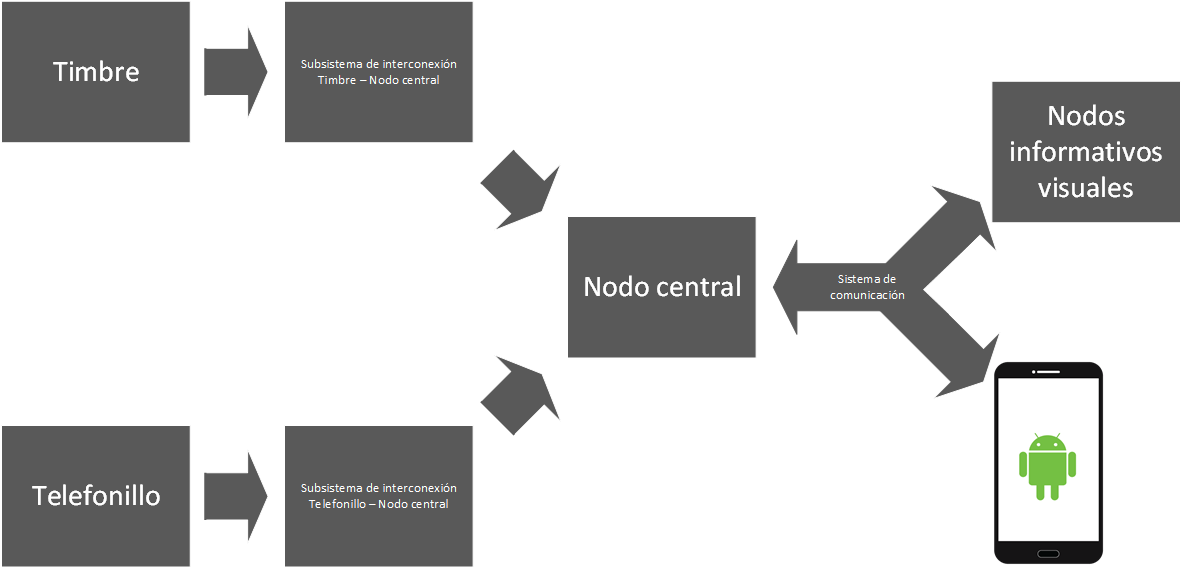
\includegraphics[width=1\textwidth]{diagrama_bloques.png}
      \caption{Diagrama de bloques del sistema.}
      \label{diagrama_bloques}
    \end{figure}

\section{Elección de los nodos informativos visuales}
    \label{sec:solucionbombillas}

    Teniendo en cuenta la tabla~\ref{tab:bombillas}, a raíz del estudio de Requisitos dentro de las Especificaciones del Sistema [~\ref{sec:especificaciones}], y sobre todo, de acuerdo con el requisito no funcional NFR-01, se busca utilizar bombillas capaces de generar luces de colores (RGB), la segunda alternativa mostrada en la tabla queda descartada, pues tan solo proporciona luz en distintos tonos de blanco (ya sea luz más cálida o más fría, y variaciones de luminosidad). \\

    Además, la tercera opción expuesta podría resultar a primera vista la solución más económica, pues permite la compra por separado del puente que comunica con las bombillas, pero debido a ser compra en el extranjero, con importantes gastos de transporte, y la imposibilidad de facturar estos gastos a través de la universidad, se descarta también esta opción. \\

    Queda claro por tanto que la opción elegida es la primera, utilizar las bombillas Hue de Philips. Estas bombillas utilizan un puente ZigBee-Ethernet, al que se conecta mediante cable Ethernet y se utiliza una interfaz propia para alterar el estado de las bombillas. Estas se controlan mediante métodos HTTP a través de una interfaz RESTful, los cuales deben recibir y generar cadenas en formato JSON, por lo que es necesario poder manipular estas cadenas de alguna manera.

\section{Elección de dispositivo de interconexión de red}

    Se ha visto la necesidad de conectar un smartphone Android al sistema (según el requisito no funcional NFR-02), y la solución más acertada para la conexión de este dispositivo parece WiFi, ya que como se ha visto, tiene mayor alcance que Bluetooth, pudiendo funcionar por tanto mucho mejor en el entorno del interior de una vivienda (teniendo en cuenta las paredes que se encuentran dentro de una vivienda). \\

    Con Bluetooth, se tiene un alcance de 10 metros, 100 en condiciones óptimas (sin obstáculos) y mediante el uso de repetidores. Con WiFi, el alcance es mucho mayor, llegando a 70-100 metros en interior, y hasta 250 metros en condiciones óptimas (en exteriores). Siendo estas dos las únicas opciones de conexión posibles para un smartphone Android, queda descartado el uso de Bluetooth, eligiendo así utilizar WiFi como medio de comunicación. \\

    Es necesario por tanto el uso de un punto de acceso WiFi al que el smartphone Android pueda conectar, comunicando así el smartphone y el nodo central. Además, para la conexión del nodo central con el puente Hue utilizado para la comunicación con las bombillas elegidas, es necesario el uso de un dispositivo que realice la función de un switch Ethernet. Debido a estas necesidades y teniendo en cuenta lo expuesto en el apartado~\ref{sec:routerintegrado} del Informe de Diagnóstico, en el que se explica que habitualmente dentro de una vivienda se cuenta con un dispositivo que cumple con estas características (un router integrado)\cite{cisco_ccna}, se decide utilizar este dispositivo para la interconexión de los tres sistemas: el nodo central, el smartphone y el puente Hue.\\

    Tanto Arduino como Raspberry Pi, las dos opciones analizadas para utilizar como nodo central, pueden lograr conexión a la red mediante un latiguillo Ethernet como solución más simple, necesitando Arduino de una placa Ethernet para lograr la conexión.

\section{Elección del nodo central}

    Tras descartar Arduino como placa programable que funcionase como nodo central, se decidió continuar con la otra alternativa estudiada: utilizar una Raspberry Pi B como nodo central. \\

    En la Raspberry Pi B se cuenta ya con interfaz de red Ethernet, por lo que no es necesario utilizar ninguna placa añadida. Además esta placa también cuenta con pines de entrada/salida programables, lo cual es indispensable para el desarrollo del Proyecto. \\

\section{Aplicación para nodo central}

    Se utilizará Python como lenguaje de programación para los programas del sistema, lenguaje cada vez más utilizado en proyectos de este tipo en los que se necesita dotar a Raspberry Pi de funcionamiento junto a sensores y otros sistemas hardware. Además, Python incluye librerías que permiten manejar cadenas JSON, establecer comunicaciones mediante peticiones HTTP, y más. Se utilizará la implementación 2.7 de Python, con soporte para todas las librerías necesarias en el Proyecto, como son las de manejo de direcciones URL.\\

    Es necesario además instalar en el sistema operativo la librería RPi.GPIO, librería externa facilitada por Python para el manejo de los pines GPIO de Raspberry Pi, necesario para la lectura del estado de los relés empleados para la detección de llamadas al telefonillo o al timbre. \\


    \subsection{Librerías desarrolladas}

        Se ha desarrollado por tanto un conjunto de programas que sean capaces de comunicarse con el puente Philips Hue mediante métodos REST y cadenas JSON (utilizadas tanto para parámetros como para respuestas del puente), detectar las alertas de las llamadas entrantes tanto de telefonillo como de timbre a través de los relés empleados para ello, y comunicarse con un dispositivo Android para replicar las mismas alertas, a modo de texto. \\
        
        Se desarrollan para ello dos librerías en Python: una para el uso de métodos REST, y otra para el control del puente Philips Hue. \\

        \subsubsection{Librería RESTful}

        Para ello, se ha desarrollado en primer lugar una librería REST en Python, que facilita la comunicación de Raspberry Pi con el puente Philips Hue. Esta librería, implementada en un único fichero, cuenta con 4 métodos principales, que serán los utilizados por el usuario: \textbf{get, post, put} y \textbf{delete}. Cada uno de ellos recibe la dirección del dispositivo al que realizar la petición, el dato a utilizar en caso de que sea necesario (POST y PUT), y el tipo de contenido del mensaje, que en este caso será siempre texto formateado en JSON. \\

        \pythonexternal[linerange={4-7,11-12,56-67}]{./contenido/src/raspberry/rest.py}
        \vspace{0.3cm}
        Además, la misma clase de la librería cuenta con un método genérico privado el cual utilizan las 4 funciones anteriores. Este método es el verdadero encargado de establecer la conexión con el dispositivo deseado, y realizar la petición REST proporcionando además los datos que sean necesarios, y recogiendo la respuesta proporcionada por el dispositivo en formato JSON. \\

        \pythonexternal[linerange={13-13,22-55}]{./contenido/src/raspberry/rest.py}
        \vspace{0.3cm}
        Lo primero que hace este método es comprobar si hay datos entrantes, si los hay, los formatea como JSON mediante la librería propia de Python, y luego comprueba el tipo de petición (PUT o POST, las dos peticiones que pueden recibir datos entrantes). \\

        Para efectuar el PUT, establece la conexión utilizando la dirección recibida, añade los datos a enviar, y la cabecera con el tipo de contenido. Finalmente realiza la petición. Por otro lado, para POST, se distinguen dos tipos: con y sin cuerpo del mensaje. Se realizan los mismos pasos, salvo que efectuando una petición POST. \\

        En cambio, si no hay datos entrantes, la petición podrá ser GET o DELETE. Se realizan las mismas acciones que en el caso anterior, solo que sin incluir datos en la petición. Finalmente, se almacena la respuesta, se cierra la conexión y se devuelve la respuesta. \\

        \subsubsection{Librería Hue}

        Por otra parte, se ha creado una librería Python para el control del puente Philips Hue, así como de las bombillas asociadas a él. Gracias a esta librería, se evita utilizar la interfaz web propia del puente, que únicamente debe utilizarse como herramienta para desarrolladores, en concreto para depuración y pruebas. Esta librería se divide en tres clases:
        \begin{itemize}
            \item Bridge: clase principal, de la que se debe crear un objeto para poder utilizar el sistema. Contendrá información como el usuario del puente Philips Hue a utilizar, o la dirección IP del mismo.
            \item Light: clase que implementa todas las funciones necesarias para el control de las bombillas, como obtener su estado o modificarlo.
            \item Config: clase que contiene funciones necesarias para la configuración del puente Philips Hue desde el mismo programa, sin necesidad de acceder a la interfaz web de depuración.
        \end{itemize}

        Estas clases están repartidas en distintos archivos.

        \paragraph{Clase Bridge}\mbox{}\\

        La clase principal de la librería está implementada en el fichero \_\_init\_\_.py del paquete de la librería, siguiendo las directrices de Python para la implementación de clases, métodos y otras funciones que se deseen ejecutar como inicialización de las librerías o paquetes creados. Esta clase principal, Bridge, cuenta únicamente con un constructor. \\

        \pythonexternal[linerange={4-14}]{./contenido/src/raspberry/__init__.py}
        \vspace{0.3cm}

        El constructor recibe la dirección IP del puente y el nombre del usuario del puente a utilizar, crea un objeto de cada una de las otras clases, Config y Light, utilizando estos parámetros; y busca en la misma inicialización bombillas que hayan sido recientemente instaladas en la vivienda, para asociarlas al puente Hue.

        \paragraph{Clase Config}\mbox{}\\

        La clase Config únicamente contiene 3 métodos relacionados con la configuración y estado del puente. Esta clase además, utiliza la librería REST anteriormente expuesta, para la comunicación con el puente. \\

        \pythonexternal[linerange={3-12,17-27}]{./contenido/src/raspberry/config.py}
        \vspace{0.3cm}

        Obviando el constructor, el cual es trivial, el primero de los métodos es un observador que comprueba si se puede conectar al puente con el usuario dado, o por el contrario, es un usuario no autorizado a utilizar dicho dispositivo. Este método realiza una petición GET a la dirección ``\textit{http://IP\_PUENTE/api/USUARIO}'', recibiendo como respuesta una cadena JSON con toda la configuración del puente si el usuario está autorizado, o un error si el usuario no está dentro de la lista de usuarios autorizados a realizar operaciones con el puente. \\

        \pythonexternal[linerange={29-29,35-39}]{./contenido/src/raspberry/config.py}
        \vspace{0.3cm}

        El segundo método recibe una cadena con el nombre de un nuevo usuario, y crea un usuario en el puente con ese nombre. De nuevo, utilizando peticiones REST, en concreto POST, se realiza la operación, resultando una cadena JSON que informará si la operación se ha realizado con éxito. \\

        \pythonexternal[linerange={41-41,47-52}]{./contenido/src/raspberry/config.py}
        \vspace{0.3cm}

        Por último, el tercer método realiza justo lo contrario que el anterior: elimina un usuario de la lista de usuarios autorizados a utilizar el puente, recibiendo como parámetro el nombre del usuario a eliminar. Mediante una petición DELETE a la dirección necesaria, se elimina ese usuario, y se devuelve información relativa al resultado de la operación.

        \paragraph{Clase Light}\mbox{}\\

        La última clase de la librería Python para Hue es Light. Esta clase implementa las funciones necesarias para controlar las bombillas Hue, como son obtener el estado de las bombillas, el número de bombillas conectadas, el estado de una bombilla individual, encontrar nuevas bombillas que conectar al puente Hue, y diversos modificadores de su estado. \\

        \pythonexternal[linerange={4-12,17-37}]{./contenido/src/raspberry/light.py}
        \vspace{0.3cm}

        Al igual que en la clase Config, el constructor es bastante trivial. El primer método de interés que se encuentra es \textbf{get}, el cual se encarga de obtener del puente Philips Hue la información de todas las bombillas conectadas, las nuevas, o una única bombilla determinada, dependiendo de la información que reciba como parámetro. Una vez controlado de qué bombilla o bombillas debe obtener la información, realiza una petición GET, y devuelve el resultado de esta operación, exceptuando si debe obtener información de todas las bombillas, caso en el que reagrupa la información de las bombillas en un vector de bombillas (vector de información de cada una de las bombillas). \\

        \pythonexternal[linerange={39-39,44-52}]{./contenido/src/raspberry/light.py}
        \vspace{0.3cm}

        El método \textbf{getNumLights} se basa en el método anterior, y a diferencia de este no recibe parámetros. Este método realiza directamente una petición GET para obtener el estado de todas las bombillas conectadas al puente, para después transformar la respuesta en un vector de bombillas, y finalmente devolver la longitud de ese vector (o lo que es lo mismo, el número de bombillas). \\

        \pythonexternal[linerange={54-54,59-61,67-67}]{./contenido/src/raspberry/light.py}
        \vspace{0.3cm}

        Los siguientes métodos, \textbf{getLightState} y \textbf{isPhisicallyOn} reciben como parámetro el número identificador de una bombilla, y utilizan internamente el método \textbf{get} expuesto anteriormente. El primero, filtra la salida de \textbf{get}, devolviendo únicamente el campo \textbf{state} del JSON generado. El segundo, hace lo mismo y además se queda solo con el parámetro \textbf{reachable} de \textbf{state}, el cual determinar si una bombilla está encendida físicamente o no (y no a través del puente Hue). \\

        \pythonexternal[linerange={69-69,73-77}]{./contenido/src/raspberry/light.py}
        \vspace{0.3cm}

        La función \textbf{findNewLights} realiza una operación parecida a \textbf{get}, cambiando que ejecuta una petición POST en lugar de GET. El resultado de realizar POST a la misma dirección mediante la cual se obtiene información de todas las bombillas con \textbf{get}, es buscar nuevas bombillas pendientes de conectar al puente, y asociarlas automáticamente a este. \\

        \pythonexternal[linerange={79-79,84-96}]{./contenido/src/raspberry/light.py}
        \vspace{0.3cm}

        Utilizado por los modificadores de estado como método base, el método \textbf{update} es un método genérico para modificar el estado de una bombilla conectada al puente Hue. Este método recibe un dato, y dependiendo de si ese dato es interno al parámetro \textbf{attr} o \textbf{state} de la bombilla, realiza la petición POST a distintas URL, junto al dato que se ha proporcionado. El resultado de este método es la modificación del estado de la bombilla, además de devolver información sobre la operación realizada. \\

        \pythonexternal[linerange={98-98,106-112,122-128,133-139,144-148}]{./contenido/src/raspberry/light.py}
        \vspace{0.3cm}

        Los últimos métodos de la clase, los modificadores de estado, son bastante simples, al utilizar internamente el método \textbf{update} genérico anterior. \textbf{setLightColor} recibe el identificador de una bombilla y los parámetros relacionados con el color, y realiza un \textbf{update} para modificar estos parámetros. \textbf{setLightState} realiza lo mismo y además, modifica también si la bombilla quedará encendida o apagada, recibiendo este atributo de estado como parámetro. Por otra parte, \textbf{setLightOn} y su contrapartida, \textbf{setLightOff} sirven para alterar el estado de encendido de la bombilla: encenderla y apagarla, respectivamente.

    \subsection{Programa principal}

        El programa principal del nodo central utiliza las librerías anteriores para conectar con el puente Philips y controlar las bombillas. Este programa además utiliza también varias librerías de Python como son \textbf{socket, sys, threading,} y la librería externa \textbf{RPi.GPIO}, entre otras.
        
        \subsubsection{Cabecera del programa y definición de variables globales}

        \pythonexternal[linerange={19-55}]{./contenido/src/raspberry/main.py}
        \vspace{0.3cm}

        En la primera parte del programa, se definen varias variables utilizadas a lo largo de este. Las cuatro primeras variables pueden modificarse, definiéndose en ellas el nombre de usuario a utilizar para conectar al puente, el idioma de los mensajes enviados al smartphone (español o inglés), y el número de los pines GPIO a los que se conectarán las señales del telefonillo y el timbre. \\

        El resto de variables definidas son variables de cadenas de caracteres en los distintos idiomas, el identificador Hue de los colores a utilizar para mostrar las alertas mediante las bombillas, la configuración de los pines GPIO, y el comando a utilizar para descubrir la dirección IP asociada al puente Hue de manera automática. Este último utiliza comandos de consola del sistema para obtener la dirección IP de la red a la que se está conectado mediante \textbf{ip route show} y varios \textbf{grep} (uno de ellos utilizando expresiones regulares para determinar el formato de la dirección IP), proporcionar ese comando a la herramienta de escaneo ARP \textbf{arp-scan}, la cual proporcionará la dirección IP de los dispositivos conectados a la red, filtrando por último el dispositivo de interés (el puente Philips Hue) para obtener únicamente su dirección IP mediante \textbf{awk}. Mientras no se obtenga la dirección del puente Hue como resultado y por tanto no se pueda conectar con él, el programa quedará iterando en estos comandos, a la espera de realizar la conexión.
        
        \subsubsection{Asociación de usuario al puente Philips Hue}

        \pythonexternal[linerange={57-69}]{./contenido/src/raspberry/main.py}
        \vspace{0.3cm}

        Entre los métodos de este programa se encuentra \textbf{linkUserConfig}, el cual se encarga de asociar el usuario configurado al puente Philips Hue si no estuviese ya creado y admitido dentro de la lista de usuarios con permisos para controlar el puente, mediante la función \textbf{createUser} de la clase Config.
        
        \subsubsection{Alerta mediante puente Philips Hue}

        \pythonexternal[linerange={71-94}]{./contenido/src/raspberry/main.py}
        \vspace{0.3cm}

        El método para mostrar las alertas a modo de parpadeo de luces de colores en las bombillas es \textbf{lightAlert}, el cual recibe el identificador de color de la alerta y comprueba si el usuario tiene permisos de conexión al puente mediante el método \textbf{isConnected} de la clase Config. Si no los tiene, se utilizará el método \textbf{linkUserConfig()} de este mismo programa. Además, al igual que se realiza al principio de la ejecución del programa al crear el objeto Bridge, se comprueba si se pueden asociar nuevas bombillas al puente Hue, para tener control en todo momento sobre todas las bombillas al alcance del puente. Tras esto se realiza una serie de operaciones para almacenar el estado previo de todas las bombillas conectadas al puente (mediante el método \textbf{getLightState} de la clase Light), cambia su estado a uno de encendido y con el color suministrado mediante parámetro, y vuelve a colocar las bombillas en su estado anterior (teniendo en cuenta si alguna de ellas estaba anteriormente apagada). Esta operación se realiza varias veces para dar un efecto de parpadeo a la alerta.
        
        \subsubsection{Alerta mediante aplicación para smartphone}

        \pythonexternal[linerange={96-112}]{./contenido/src/raspberry/main.py}
        \vspace{0.3cm}

        El último de los métodos secundarios del programa principal, \textbf{sendAlertToAndroid} es el encargado de quedar a la espera de conexiones entrantes mediante el socket establecido en el método principal del programa. Si se recibe una petición, se controla que es una petición válida (deberá contener el texto ``/getAlert''), y se envían los datos definidos en el programa hacia el smartphone, utilizando la dirección IP que realizaba la petición, y el puerto 8081. Si la petición no es válida, se generará un mensaje de error y se enviará de la misma manera. \\

        Es ya en la función \textbf{main()} donde se realizan los últimos ajustes e inicializaciones para que el sistema se ponga en marcha, y donde se desarrolla la ejecución principal del programa.
        
        \subsubsection{Método principal del programa}

        \pythonexternal[linerange={114-151}]{./contenido/src/raspberry/main.py}
        \vspace{0.3cm}

        En este método se crea un socket UDP en el puerto 8080, el cual será el encargado de recibir peticiones de nuevas alertas desde el smartphone, y enviar estas alertas hacia el dispositivo. \\

        A continuación, se obtiene la dirección IP del puente Hue con la secuencia de comandos anteriormente descrita, y se crea un objeto de la clase Bridge (el cual creará a su vez una instancia de las clases Config y Light), para poder comunicar este programa con el puente. Tras ajustar las variables de mensajes al idioma seleccionado, se inicia un hilo que tendrá como objetivo el método \textbf{sendAlertToAndroid()}. \\

        Una vez que está listo todo lo anterior, empieza la iteración sin pausa de la parte principal de este programa. Se comprueban los pines GPIO asociados al timbre y al telefonillo, con el objetivo de detectar alertas generadas por estos. De realizar una lectura positiva de alerta, se ejecuta la función \textbf{lightAlert} con el color asociado al tipo de alerta, estableciendo como parámetro la fecha y hora de la alerta, junto con una cadena de texto a mostrar en el smartphone. \\

    \subsection{Estructura final de ficheros}

        En la figura~\ref{dirs} se muestra la estructura final de directorios y ficheros del software implementado para el nodo central.

        \begin{figure}[!ht]
          \centering
            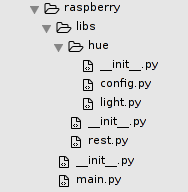
\includegraphics[width=0.35\textwidth]{dirs.png}
          \caption{Estructura de directorios y ficheros del software del nodo central.}
          \label{dirs}
        \end{figure}

\section{Elección de electrónica para la detección de alertas}
\label{sec:sistemas_interconexion}

    Teniendo en cuenta la facilidad que supone el uso de relés y la sencillez de su montaje electrónico e inclusión en el sistema, se opta por esta opción.

    \subsection{Detección de alertas del telefonillo}

    Para la detección de alertas por parte del telefonillo, se utiliza un relé de 12 Vac para detectar las llamadas. Este relé se conecta, por la toma de entrada, a la salida del telefonillo (la salida de su interruptor) y a corriente eléctrica de 12 Vac. La salida del relé se conecta al nodo central (la Raspberry Pi), conectando un extremo a un pin GND del GPIO (en concreto el pin 9 de la numeración física~\cite{raspberrypigpio}) y el otro, mediante resistencia de pull-up de 4,7 K$\Omega$, al pin 18 GPIO (de numeración GPIO) y a una salida de corriente de 3,3 V (pin 17 de la numeración física~\cite{raspberrypigpio}), tal como se observa en la figura~\ref{circuitotelefonillo}.\\

    \begin{figure}[!ht]
      \centering
        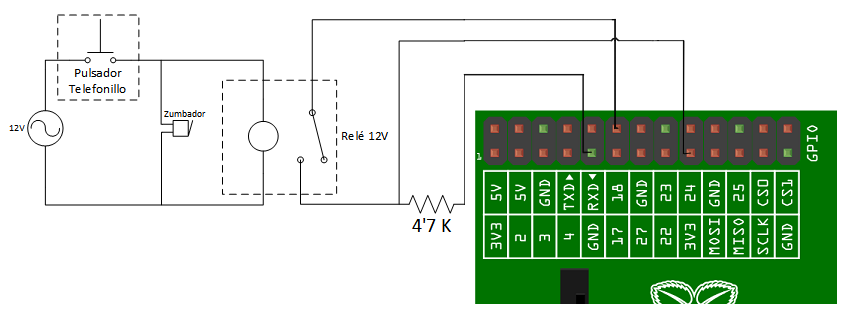
\includegraphics[width=0.75\textwidth]{circuitotelefonillo.png}
      \caption{Diseño del circuito de interconexión telefonillo-nodo central.}
      \label{circuitotelefonillo}
    \end{figure}
    
        \subsubsection{Implementación}
    
        Para la implementación de este circuito en el sistema, se crea una placa de circuito impreso (PCB) con los componentes y conexionado necesario. El esquemático y el diseño del layout de esta PCB se encuentran en el documento de Planos, en los planos número 1 (apartado~\ref{sec:plano1}) y número 2 (apartado~\ref{sec:plano2}), respectivamente. \\
        
        Teniendo en cuenta que el consumo del telefonillo no supera los 2 A de corriente, a un voltaje de 12 V, y utilizando una longitud de pistas de entrada al relé de 2 cm, se calcula que el ancho de las pistas que soporte esta tensión debe ser como mínimo de 780 $\mu$m. \\
        
        Por otro lado, al conectarse esta PCB a los pines GPIO de Raspberry Pi, que generan una corriente de 3,3 V a 50 mA~\cite{raspberry_pinout}, y suponiendo que estas placas de circuito impreso se sitúen a una distancia estimada de 30 m de la Raspberry Pi, utilizando cableado de 20 AWG de diámetro se obtendría una caída de voltaje de 51,35 mV (1,56 \%), lo que supone una caída de voltaje despreciable, obteniendo un voltaje final de entrada al pin GPIO de Raspberry Pi de 3,25 V.

    \subsection{Detección de alertas del timbre}

    Para la detección de las alertas producidas por llamadas al timbre, se utiliza un relé de 230 Vac. Este relé se conecta, por la toma de entrada, a la salida del timbre (la salida de su interruptor) y a corriente eléctrica de 230 Vac. A su vez, la salida del relé se conecta a la Raspberry Pi conectando un extremo a un pin GND del GPIO (en concreto el pin 6 de la numeración física~\cite{raspberrypigpio}) y el otro, mediante resistencia de pull-up de 4,7 K$\Omega$, al pin 17 GPIO (de numeración GPIO) y a una salida de corriente de 3,3 V (pin 1 de la numeración física~\cite{raspberrypigpio}), tal como se observa en la figura~\ref{circuitotimbre}.\\

    \begin{figure}[H]
      \centering
        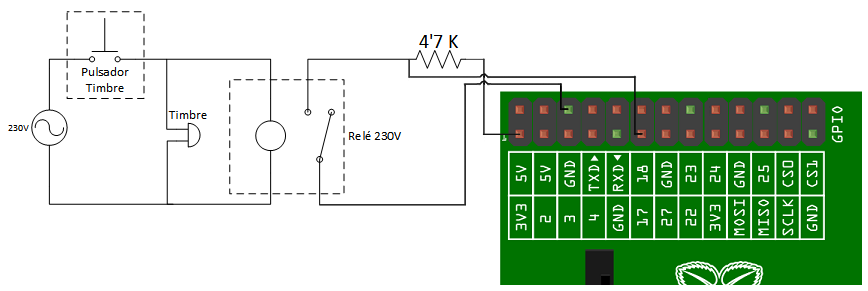
\includegraphics[width=0.8\textwidth]{circuitotimbre.png}
      \caption{Diseño del circuito de interconexión timbre-nodo central.}
      \label{circuitotimbre}
    \end{figure}
    
        \subsubsection{Implementación}

        Para la implementación de este circuito en el sistema, se crea una placa de circuito impreso (PCB) con los componentes y conexionado necesario. El esquemático y el diseño del layout de esta PCB se encuentran en el documento de Planos, en los planos número 3 (apartado~\ref{sec:plano3}) y número 4 (apartado~\ref{sec:plano4}), respectivamente. \\
        
        Teniendo en cuenta que el consumo del timbre no supera los 0,2 A de corriente, a un voltaje de 220 V, y utilizando una longitud de pistas de entrada al relé de 2,5 cm, se calcula que el ancho de las pistas que soporte esta tensión debe ser como mínimo de 32 $\mu$m. \\
        
        Por otro lado, el cálculo de caída de voltaje se realiza de la misma manera que para la placa anterior, y utilizando el mismo cableado resulta el mismo porcentaje de caída de voltaje, 1,56 \%, suponiendo que la entrada del telefonillo a la vivienda también se sitúe a 30 m de la Raspberry Pi y por tanto se ubique ahí esta placa de circuito impreso.
        
\section{Integración del sistema}

    Para la integración del sistema completo, el nodo central tendrá que comunicar con el resto de dispositivos y sistemas que conforman el sistema final, siendo el nodo central la Raspberry Pi, y los nodos subyacentes los sistemas de interconexión con el telefonillo y el timbre (de los que recibirá información el nodo central), el puente Philips Hue y el smartphone Android, con los que se comunicará a través del router integrado y se recibirá información además de enviar alertas hacia ellos. \\

    \begin{figure}[H]
      \centering
        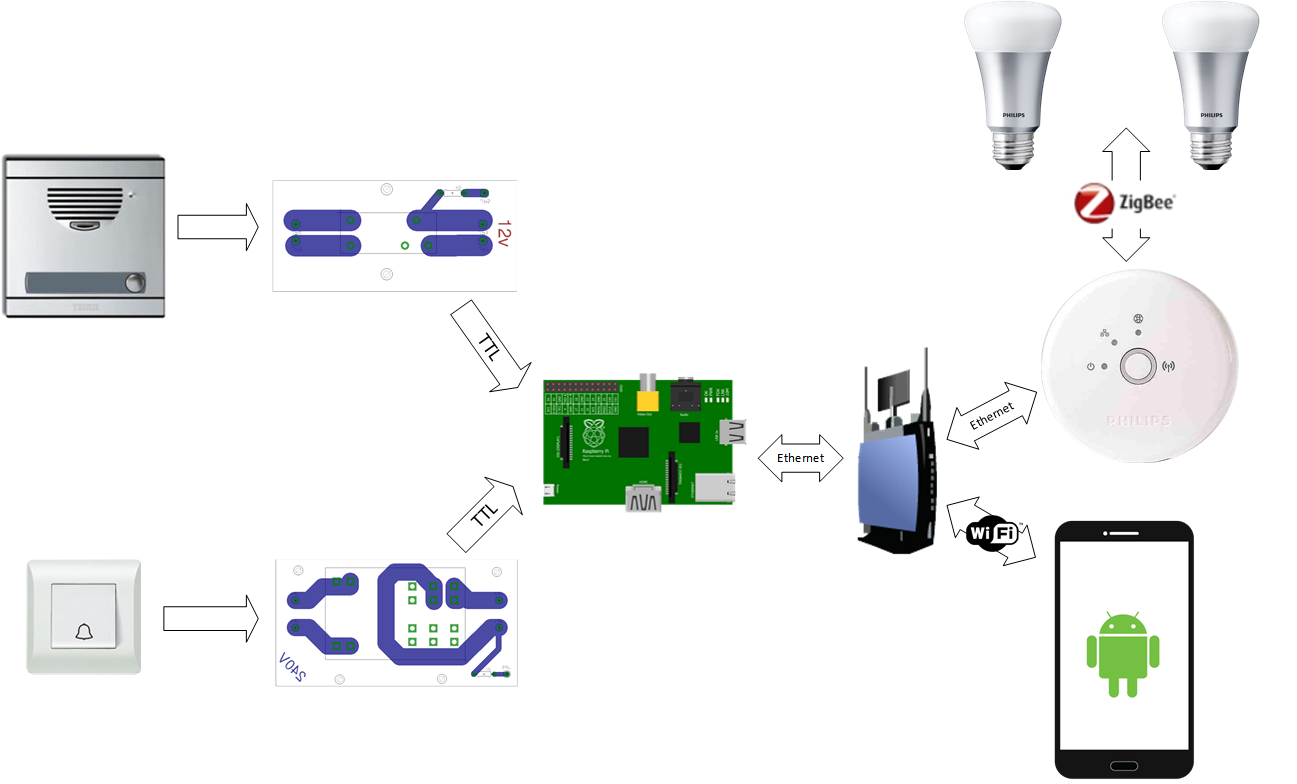
\includegraphics[width=0.9\textwidth]{integracion_sys.png}
      \caption{Diagrama de integración del sistema con el nodo central.}
      \label{integracion_sys}
    \end{figure}
    
     Complementando este diagrama, en la figura~\ref{diagrama_arquitectura} se puede observar el diseño final del sistema de forma detallada, incluyendo todos los elementos que lo conforman, una vez se ha definido el conexionado entre los sistemas de interconexión, el nodo central, el puente Philips Hue y el smartphone. \\

    \begin{figure}[H]
      \centering
        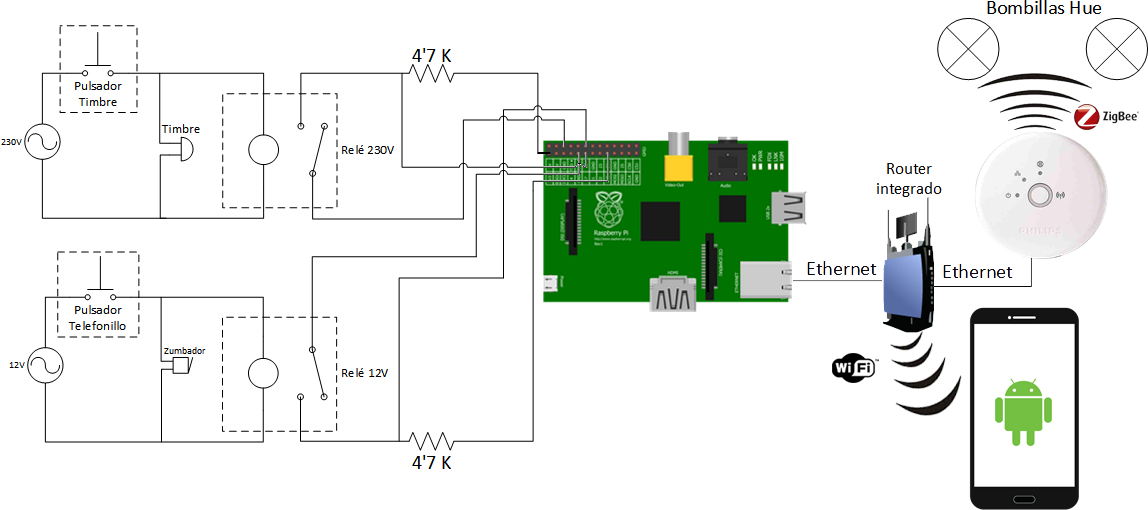
\includegraphics[width=1\textwidth]{diagrama_arquitectura.png}
      \caption{Diseño final de la arquitectura del sistema.}
      \label{diagrama_arquitectura}
    \end{figure}

\section{Aplicación para Android}

    \subsection{Diseño de la aplicación}

    El diseño de la aplicación sigue las normas de diseño de Google, utilizando una interfaz basada en MaterialDesign. Tras realizar un diseño de prototipo, el cual se puede observar en el apartado~\ref{sec:disenoapp}, previo al uso del IDE Android Studio, se decide basar el estilo general de la aplicación en el predeterminado generado por Android Studio al utilizar MaterialDesign como base. En cada pantalla de la aplicación se encuentra la barra superior de la aplicación, ActionBar, en la que se encuentra el acceso al menú de configuración o el botón de vuelta a la pantalla anterior, según la vista en la que se encuentre el usuario. En la figura~\ref{app1} se puede observar la pantalla principal de la aplicación. \\

    \begin{figure}[H]
      \centering
      {%
        \setlength{\fboxsep}{0pt}%
        \setlength{\fboxrule}{1pt}%
        \fbox{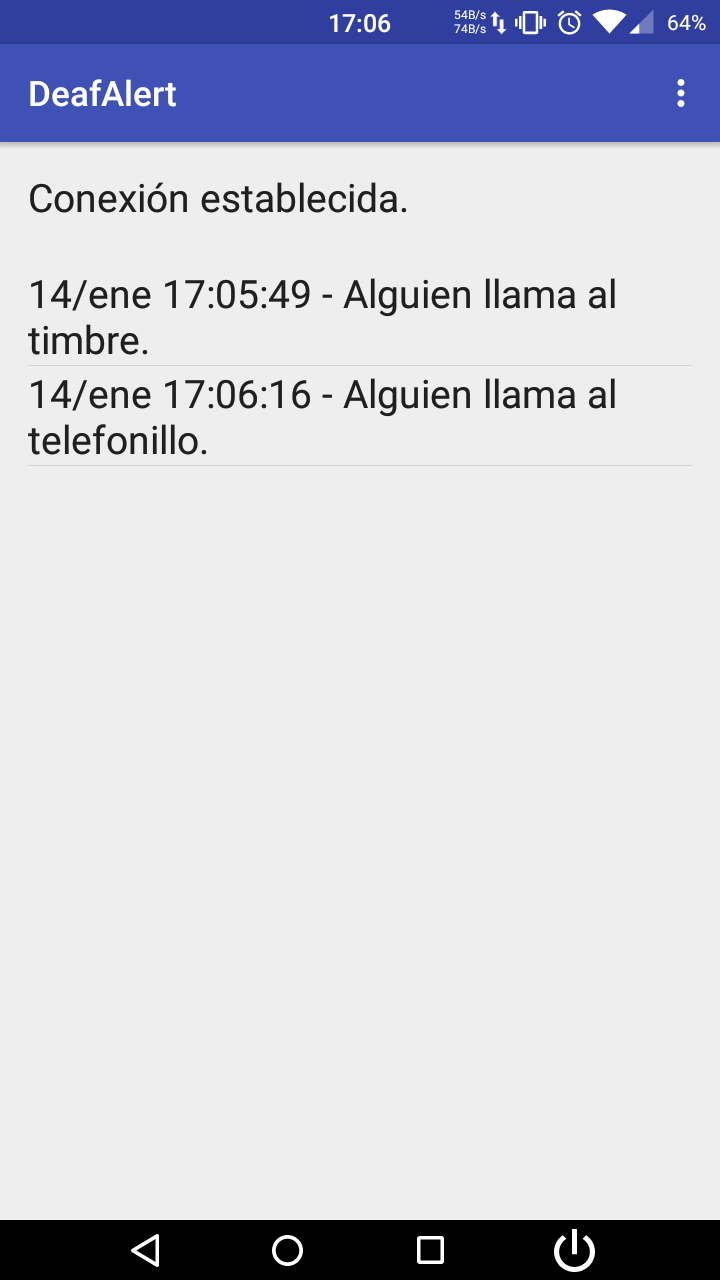
\includegraphics[width=0.3\textwidth]{app1.png}}
      }%
      \caption{Pantalla principal de la aplicación para Android.}
      \label{app1}
    \end{figure}

    En esta pantalla principal se encuentra la lista de alertas recibidas desde el servidor de alertas (la Raspberry Pi), además de un texto que indica el estado de conexión o de alertas entrantes. Tal como se muestra en la figura~\ref{app2}, estas alertas pueden ser eliminadas a mano desde la propia aplicación, de tal manera que cuando el usuario pulsa en una de ellas, la aplicación mostrará un mensaje preguntando si se desea eliminar la alerta. \\

    \begin{figure}[!ht]
      \centering
      {%
        \setlength{\fboxsep}{0pt}%
        \setlength{\fboxrule}{1pt}%
        \fbox{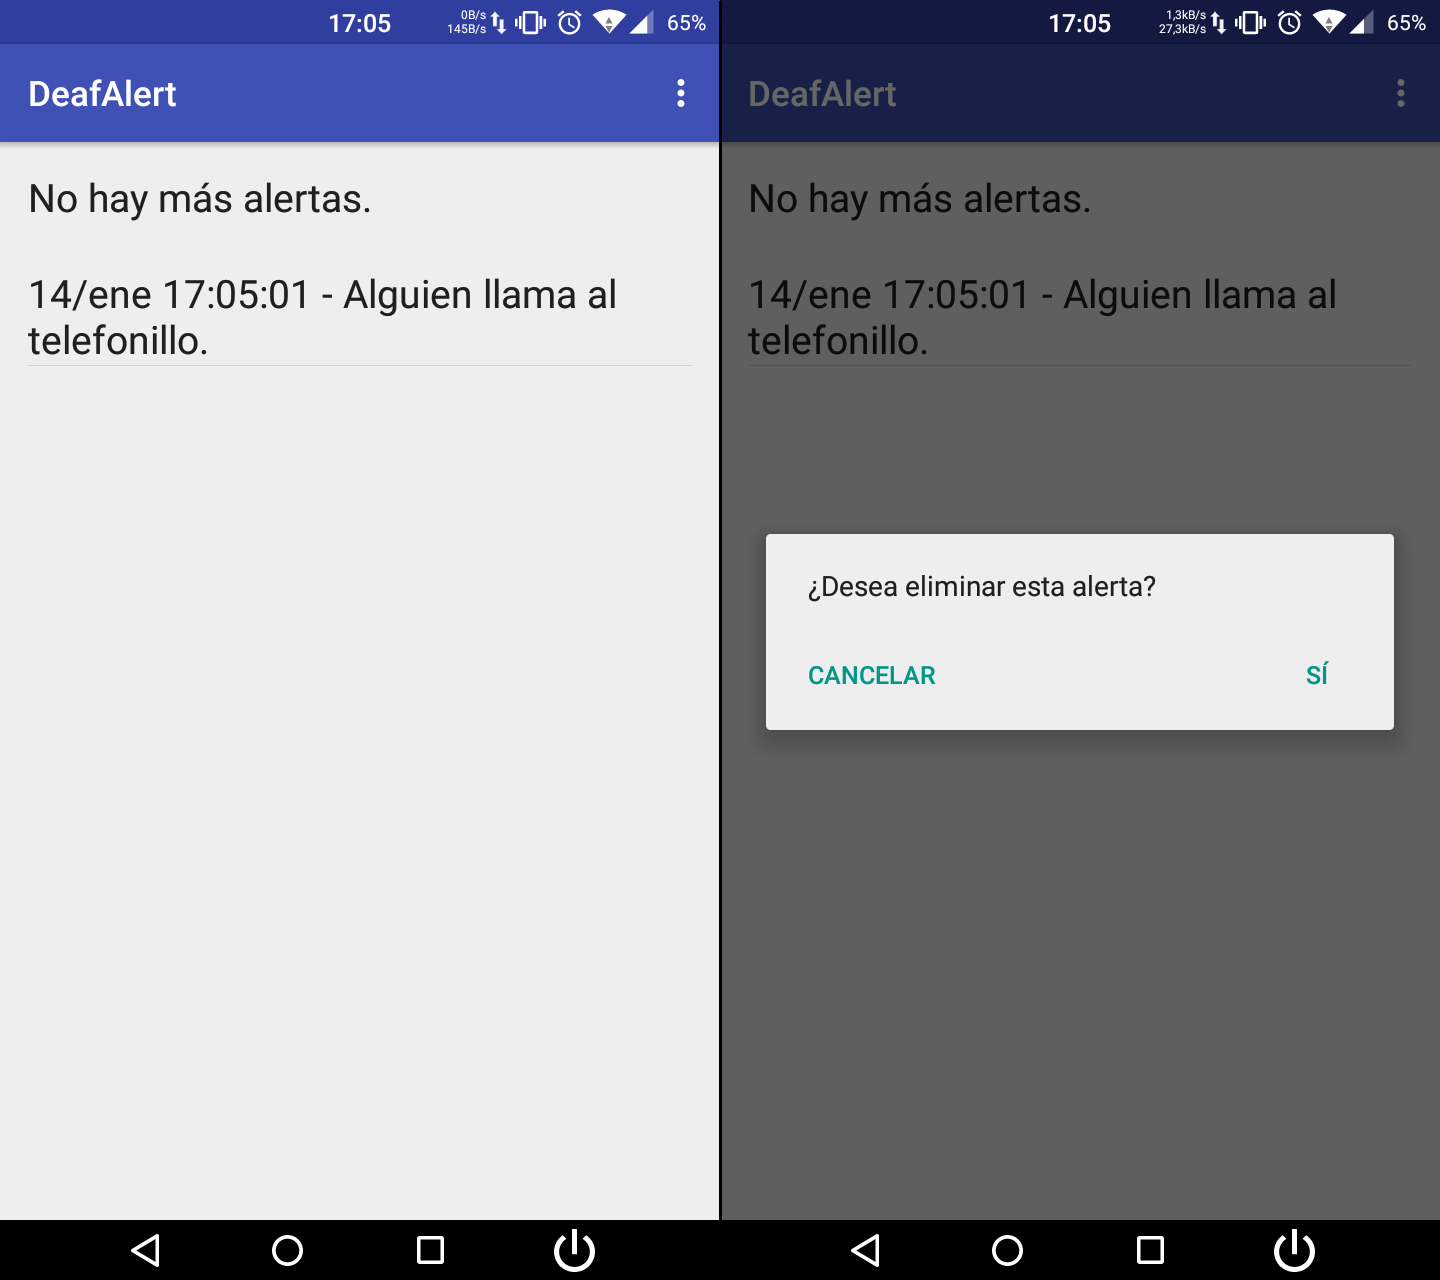
\includegraphics[width=0.6\textwidth]{app2.png}}
      }%
      \caption{Borrado de alertas en aplicación para Android.}
      \label{app2}
    \end{figure}

    Además de esta pantalla principal, la aplicación cuenta con un menú de configuración, fácilmente accesible mediante el menú desplegable superior, donde se puede configurar la dirección IP del servidor de alertas, tal y como se observa en la figura~\ref{app3}.

    \begin{figure}[H]
      \centering
      {%
        \setlength{\fboxsep}{0pt}%
        \setlength{\fboxrule}{1pt}%
        \fbox{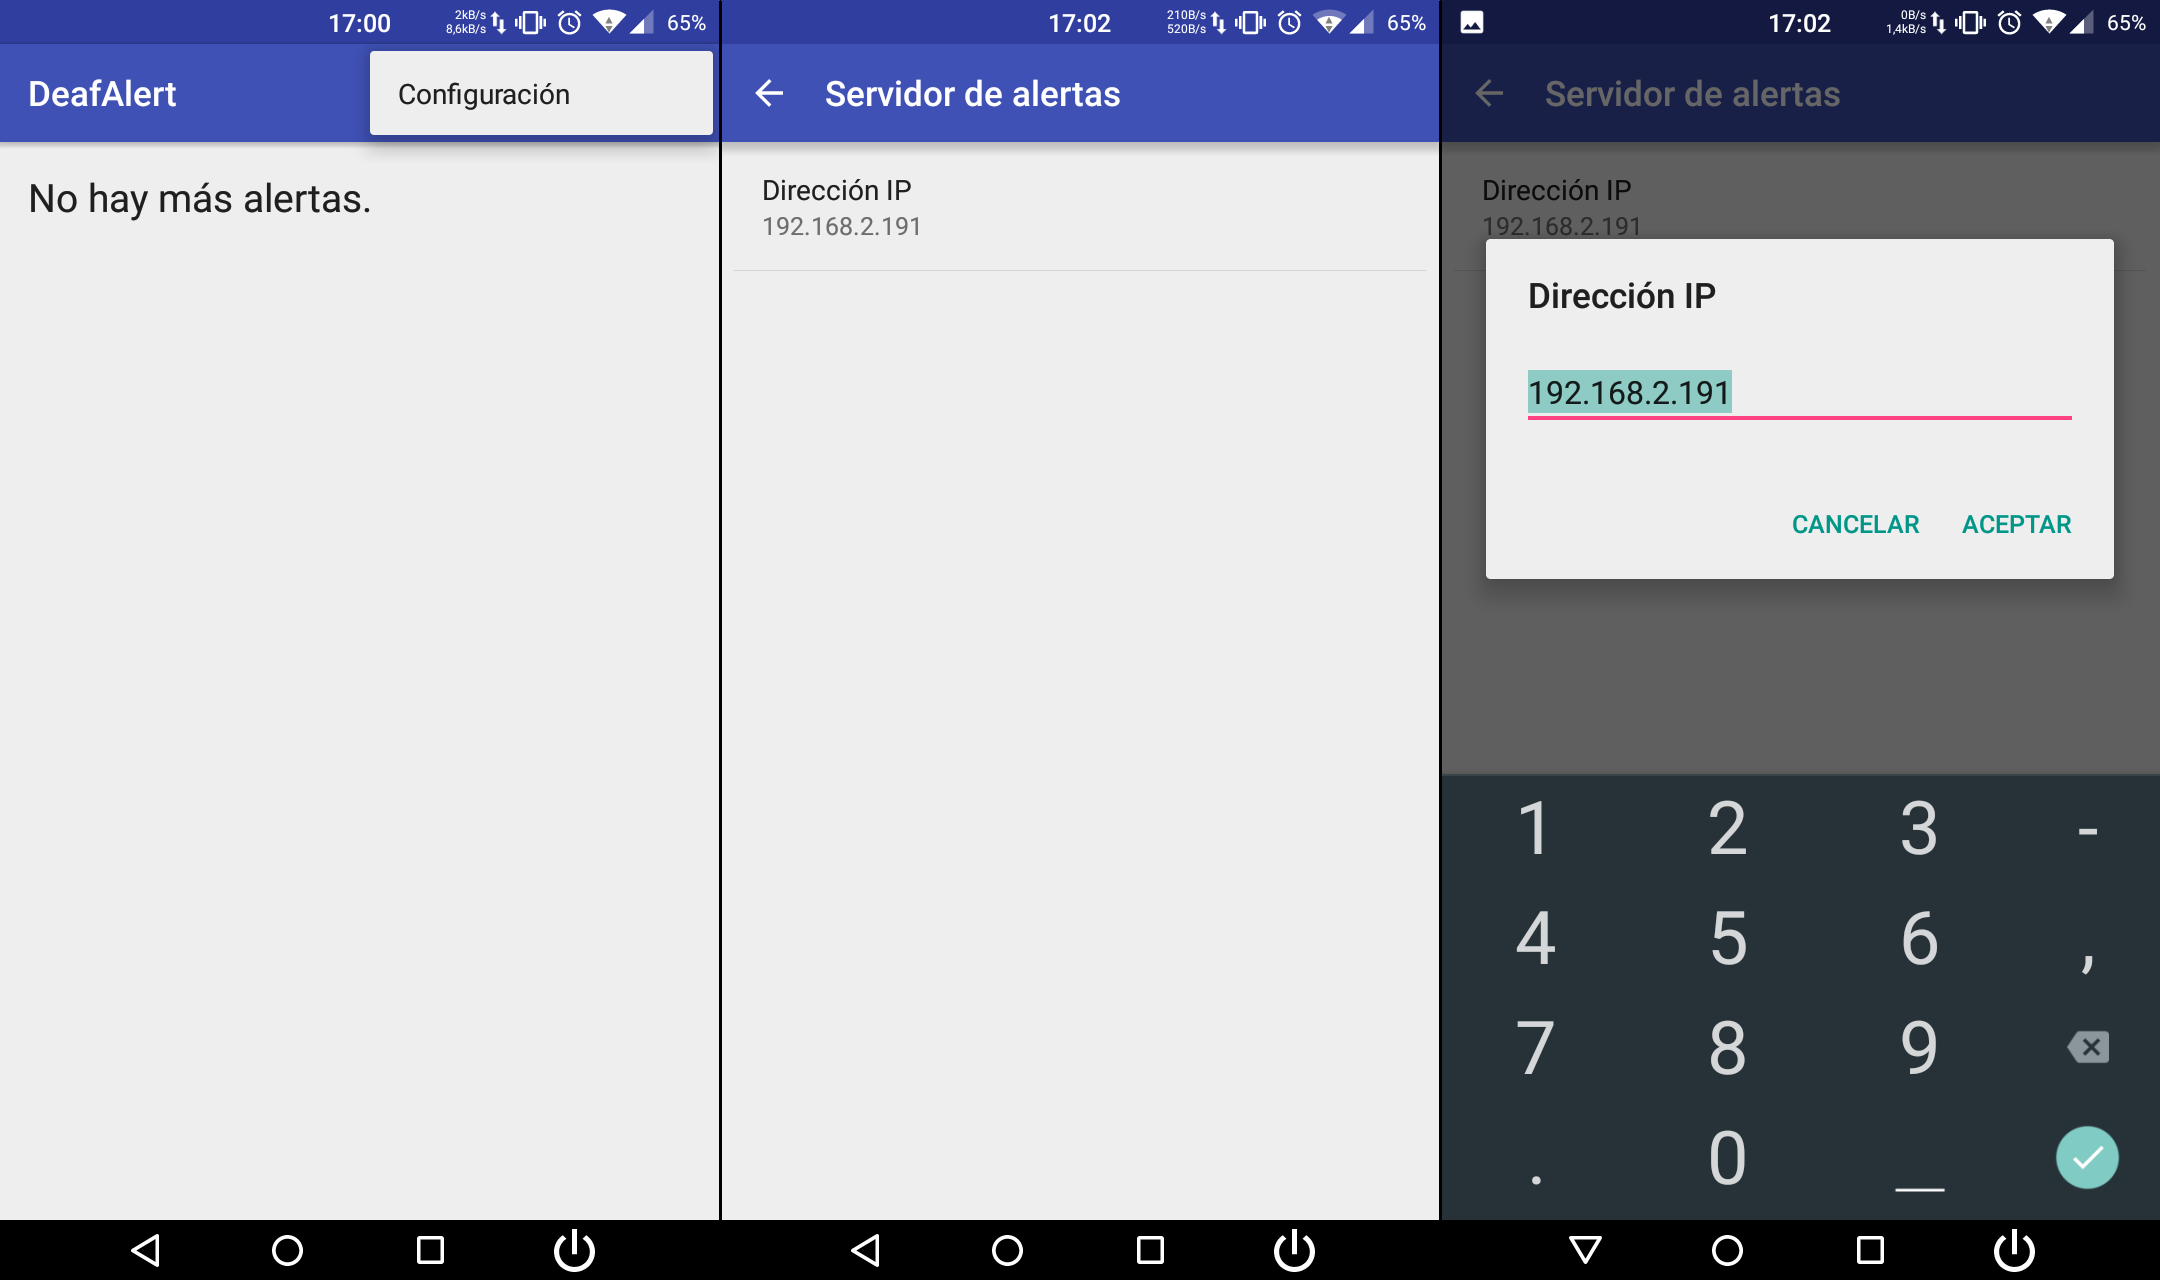
\includegraphics[width=0.8\textwidth]{app3.png}}
      }%
      \caption{Menú de configuración de aplicación para Android.}
      \label{app3}
    \end{figure}

    \subsection{Estructura software principal}

    La aplicación Android, desarrollada con el IDE Android Studio, se basa en tres clases java principales, divididas en archivos del mismo nombre:

    \begin{itemize}
        \item \textbf{MainActivity}: Clase principal de la aplicación, encargada de construir la vista principal de la aplicación Android, y dar funcionalidad a la misma. Es además la encargada de comunicar con el nodo central, tratar las alertas y mostrarlas en la pantalla principal.
        \item \textbf{AlertListAdapter}: Clase utilizada por MainActivity, para controlar la lista de alertas entrantes e ir refrescando la vista principal de la aplicación con esas alertas.
        \item \textbf{SettingsActivity}: Clase generada por el propio IDE, la cual implementa el menú de configuración de la aplicación, modificada para dotar a la aplicación de un menú de configuración que se adapte a las necesidades.
    \end{itemize}

    Además de estas clases java, la aplicación cuenta con otra clase java más generada por Android Studio, la cual no se analizará, pues es código generado automáticamente.

        \subsubsection{Actividad principal}

        En la actividad principal (MainActivity) es donde se desarrolla la funcionalidad principal de la aplicación, y es la encargada de generar la vista principal de la misma (la vista a la que se accede una vez se abre la aplicación).

        \androidexternal[linerange={35-68}]{./contenido/src/android/MainActivity.java}
        \vspace{0.3cm}

        Esta clase cuenta con varios atributos necesarios para almacenar la dirección IP del servidor de alertas, referencias a partes de la vista principal, una lista de cadenas que constituyen las alertas, un adaptador para estas alertas que será el encargado de refrescar las vistas, y otros atributos utilizados para control de notificaciones. \\

        La función principal de la clase y por tanto de la actividad es el método \textbf{onCreate}, el cual se encarga de dotar de funcionalidad a la aplicación cuando la vista principal es cargada. Además de inicializar algunos de los atributos anteriormente citados con valores predeterminados establecidos en la aplicación, se establece un objeto \textbf{AlertListAdapter} asociado a la actividad y a la lista de alertas. Una vez que esto está hecho, se crea un objeto de la clase Timer, el cual se encarga de ejecutar un método determinado cada cierto periodo de tiempo. Este método es \textbf{printRaspberryData}, el cual se examinará más adelante. \\

        Con todos los atributos inicializados y el Timer puesto en marcha, se establecen las políticas de la aplicación y se pone esta en funcionamiento. \\

        \androidexternal[linerange={124-125,147-209}]{./contenido/src/android/MainActivity.java}
        \vspace{0.3cm}

        El método \textbf{printRaspberryData} tiene un funcionamiento bastante sencillo, el cual se limita a establecer un objeto de tipo Runnable para el hilo principal de la interfaz de la aplicación. \\

        Es en este objeto Runnable donde se desarrolla el funcionamiento principal de la aplicación. En él se establece el comportamiento del método \textbf{run()}, método asociado a cada ejecución del hilo. Lo primero que realiza este método es comprobar la conexión WiFi del dispositivo. Si este no está habilitado, muestra un mensaje de error y sale del método, esperando a la próxima ejecución de este método a raíz del Timer establecido en \textbf{onCreate} para comprobar de nuevo si la conexión WiFi ha sido habilitada. \\

        Una vez el dispositivo cuente con conexión WiFi, se obtienen las preferencias almacenadas en el contenedor SharedPreferences de la aplicación. De estas preferencias se obtiene la dirección IP del servidor de alertas del que recibir las mismas. \\

        A continuación, se crea un objeto \textbf{DatagramSocket}, un socket de conexión UDP, el cual se configura para conectar a la dirección del servidor de alertas (la Raspberry Pi) a través del puerto 8080. Además se establece el puerto de escucha de datos entrantes en el puerto 8081. Si la conexión se lleva a cabo correctamente, se realiza una petición con el dato asociado ``GET /getAlert'', incluyendo este mensaje en un objeto \textbf{DatagramPacket}, paquete UDP que será enviado a través del socket. \\

        Si el envío surte efecto, se crea un nuevo objeto DatagramPacket, pero esta vez no será enviado, sino que servirá para almacenar los datos entrantes. A continuación, el hilo queda a la espera de alguna conexión entrante a través del socket. Una vez hay datos entrantes, el paquete se almacena en el objeto creado anteriormente, se extrae el dato (la alerta), y se añade a la lista de alertas, mostrándola por pantalla a través del objeto \textbf{AlertListAdapter}. Además, se muestra un mensaje de conexión satisfactoria en la aplicación, y si la aplicación estuviera en segundo plano o el dispositivo se encontrase en modo reposo (bloqueado), se envía una notificación al sistema con la alerta entrante. El comportamiento del objeto AlertListAdapter, así como lo que ocurre con la lista de alertas, se tratan en el apartado~\ref{sec:alertlistadapter}. \\

        \androidexternal[linerange={90-116}]{./contenido/src/android/MainActivity.java}
        \vspace{0.3cm}

        Además, en el método \textbf{onResume} se establece el comportamiento de la app cuando se pulse en alguna de las alertas de la lista, utilizando para ello el método \textbf{OnItemClickListener} de la clase AdapterView, el cual crea una instancia de un objeto de escucha de clicks en items o elementos de la lista. Redefiniendo el método \textbf{onItemClick} se establece este comportamiento. En primer lugar, se crea un objeto AlerDialog.Builder, el cual se encargará de generar un diálogo emergente de alerta. A continuación se establecen el mensaje del diálogo (mediante el método \textbf{setMessage}), la funcionalidad al pulsar el botón ``Cancelar'', el cual simplemente saldrá del diálogo de alerta, y la funcionalidad del botón ``Sí'', el cual eliminará la alerta de la lista. Finalmente, se genera el objeto de alerta y se muestra la alerta mediante el método \textbf{show}. \\

        \androidexternal[linerange={70-88}]{./contenido/src/android/MainActivity.java}
        \vspace{0.3cm}

        Por otro lado, mediante el método \textbf{onCreateOptionsMenu} se establece el menú de la aplicación, generando un botón para acceder al menú mediante el método \textbf{getMenuInflater}. \\

        Además, se dota de funcionalidad al menú con el método \textbf{onOptionsItemSelected}, donde se asocia cada elemento del menú con una actividad a iniciar (una nueva vista de la aplicación). Esto se realiza mediante el uso de objetos de la clase Intent, asociando en este caso una instancia de esta clase a la clase SettingsActivity, clase que implementa la actividad del menú, que se expone en el apartado~\ref{sec:menuapp}. A continuación, se inicia la actividad por medio de este objeto Intent. \\

        \androidexternal[linerange={126-146}]{./contenido/src/android/MainActivity.java}
        \vspace{0.3cm}

        Finalmente, el último método de la actividad principal, \textbf{notifyAlertToNotification}, utilizado en el hilo Runnable explicado anteriormente, es el encargado de generar y enviar notificaciones al sistema. Lo primero que se realiza en esta función es crear un objeto Builder de la clase NotificationCompat, el cual se inicializa con una serie de opciones para la notificación, como son el icono de la notificación, el título, el texto que debe contener, y distintos tipos de alerta como el color con el que el led del smartphone debe parpadear, la vibración, y cómo generar estas alertas. De este modo, la persona que utilice la aplicación podrá sentir mediante vibración o notar visualmente la alerta mediante el led, sin necesidad de tener el dispositivo desbloqueado. \\

        Tras crear este objeto, se crea una instancia de la clase Intent asociada a la actividad principal de la aplicación, y mediante un objeto de la clase TaskStackBuilder, se asigna el camino de vuelta al pulsar el botón ``Volver'' del propio dispositivo. A continuación, mediante un objeto de la clase NotificationManager se obtiene el servicio del sistema relacionado con las notificaciones, y se notifica la alerta mediante el método \textbf{notify} propio de esa clase, utilizando un número de identificación para la notificación, y el objeto builder creado al principio de la función.


        \subsubsection{Gestión de alertas}
        \label{sec:alertlistadapter}

        La gestión de las alertas a mostrar en la aplicación, así como la funcionalidad de refrescar las mismas en la lista de alertas dentro de la vista principal, se realiza mediante la clase \textbf{AlertListAdapter}, clase que hereda de la clase BaseAdapter, clase java de Android utilizada para actualizar el contenido de una vista ListView, vista utilizada en la vista principal para mostrar la lista de alertas. \\

        \androidexternal[linerange={15-23,69-72}]{./contenido/src/android/AlertListAdapter.java}
        \vspace{0.3cm}

        El constructor de la clase recibe un objeto Activity, la actividad asociada al Adapter, y un ArrayList de String, la lista de alertas. Mediante la instancia de Activity obtiene un objeto Inflater, necesario para obtener más adelante el objeto ListView a actualizar. \\

        Además, se crea una subclase ViewHolder, la cual incluye un objeto de tipo TextView, tipo utilizado para generar cada elemento de la lista ListView. \\

        \androidexternal[linerange={58-67}]{./contenido/src/android/AlertListAdapter.java}
        \vspace{0.3cm}

        Los métodos encargados de manipular la lista son \textbf{setData} y \textbf{remove}. El primero recibe una cadena con la alerta, la almacena en la lista, y mediante el método \textbf{notifyDataSetChanged} actualiza la información mostrada en la vista principal, refrescando el ListView asociado. El segundo método elimina un elemento de la lista y luego notifica de igual manera el cambio. \\

        \androidexternal[linerange={40-55}]{./contenido/src/android/AlertListAdapter.java}
        \vspace{0.3cm}

        Es necesario además sobrecargar el método \textbf{getView} de BaseAdapter, para poder obtener la vista a modificar cuando se deba actualizar el contenido de la lista de alertas. Este método usa un objeto de tipo View y otro de la subclase creada anteriormente, ViewHolder. Primero se obtiene el layout o vista a modificar de la apliación mediante el Inflater obtenido en el constructor, para a partir de esta referencia obtener la vista interna que actualizar, mediante su identificador. Hecho esto, ya se puede incluir el texto de la alerta en el TextView asociado al objeto ViewHolder utilizado.

        \subsubsection{Menú de configuración}
        \label{sec:menuapp}

        El menú de configuración está basado en el menú generado por Android Studio. Este menú incluye opciones sobrantes, por lo que se retiran todas las partes sobrantes dejando un único submenú con un campo de texto a rellenar, para configurar la dirección IP del servidor de alertas. \\

        Este menú se implementa mediante la clase SettingsActivity, el cual incluye subclases en su interior que heredan de la clase PreferenceFragment (propia del SDK de Android) por cada submenú. En este caso, al haber un único submenú, hay una única subclase, \textbf{ServerAlertsPreferenceFragment}. \\

        \androidexternal[linerange={141-168,179-179}]{./contenido/src/android/SettingsActivity.java}

        Esta clase cuenta con una constante de la clase Pattern, una plantilla, que define como debe estar formada una dirección IP, para poder comparar la preferencia establecida con esta plantilla, y así su validez. \\

        Es en el método \textbf{onCreate} donde se genera el campo para establecer la dirección IP. A continuación se genera una vista de texto para preferencias (EditTextPreference). Una vez hecho, se obtiene la preferencia con identificador \textbf{ip\_address}, y se establece una escucha para cuando el valor de esta preferencia cambie, con el método \textbf{setOnPreferenceChangeListener}. Como parámetro de este método, se crea un objeto \textbf{onPreferenceChangeListener}, para el cual se redefine la función onPreferenceChange. \\

        Esta función será la encargada de quedar a la espera de un cambio en el valor de la preferencia, comprobando cuando esto ocurra, si el valor es una dirección IP válida, mediante el método \textbf{matcher} de la clase Pattern. Finalmente, se almacena el valor de la preferencia mediante el método \textbf{bindPreferenceSummaryToValue}.


\chapter{Planificación Temporal}

La planificación temporal del Proyecto se basa en el tiempo que ha tomado realizar el Trabajo de Fin de Grado que envuelve este Proyecto, desde la toma de contacto con el director del Proyecto, hasta la finalización del mismo. La planificación se divide en varias etapas, pasando por el estudio de la situación actual y la elicitación de requisitos, investigación y búsqueda de información sobre los distintos dispositivos y distintas tecnologías a utilizar en el Proyecto y estudiando las alternativas que surgieran. Finalmente, teniendo claro todo el estudio realizado, se comienzan algunas pruebas, tras concretar las especificaciones del sistema y los requisitos del mismo. Se decidió la comunicación a emplear en todo el sistema, así como la utilizada entre los nodos informativos visuales y los dispositivos generadores de alertas. \\

Tras las pruebas realizadas, y descartando finalmente el uso de una de las alternativas para nodo central, Arduino, se comienza a realizar el sistema final, teniendo ya avanzado gran parte del trabajo gracias a todo el estudio e investigación anterior. Simultáneamente a todo lo anterior, se va generando también la documentación del Proyecto, realizando recurrentemente las modificaciones en la misma para que fuese acorde con las soluciones tomadas y los estudios realizados.

\begin{figure}[!ht]
    \centering
    {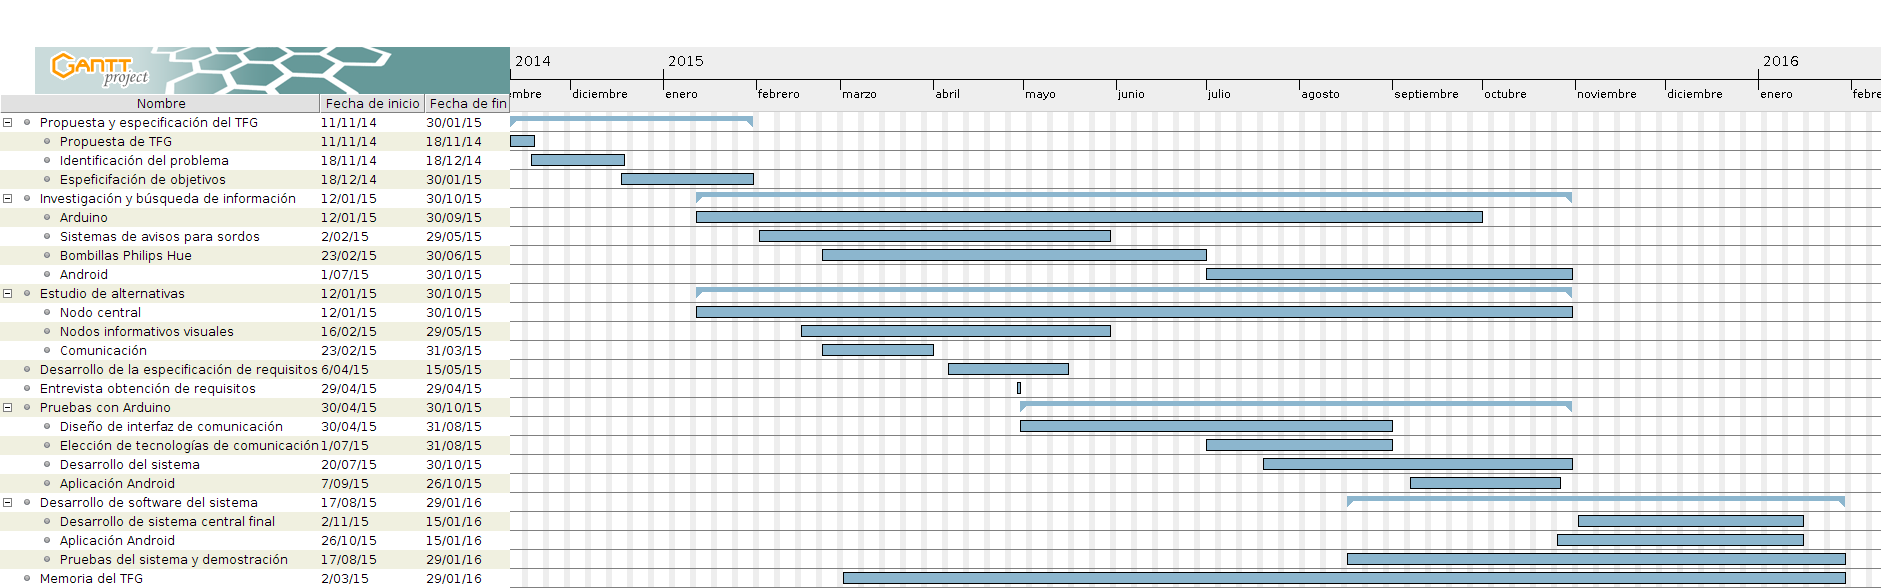
\includegraphics[width=1.15\textwidth,angle=90]{diagramagantt.png}}
        \caption{Diagrama de Gantt de la planificación temporal del Proyecto}
        \label{diagramagantt}
\end{figure}

\clearpage

\chapter{Resumen del Presupuesto}
Los costes de presupuesto para la implantación en una vivienda real son de 277.08 €, debiéndose sumar además el coste de mano de obra, que asciende a los 130 €. Esto supone un \textbf{coste total de 407.08 €}. Se debe tener en cuenta además que este precio es el relativo a instalar 3 bombillas Hue, teniendo un coste de 52.99 € por bombilla extra a instalar~\cite{hueindividualprice}, tal como se muestra en la tabla~\ref{tab:resumenpresupuesto}.

    \begin{table}[!ht]
        \centering
        \resizebox{0.6\textwidth}{!}{%
        \begin{tabular}{|l|c|}
            \hline
            \textbf{Descripción} & \textbf{Precio} \\ \hline
            Implantación del Proyecto en vivienda real & 277.08 €\\ \hline
            Mano de obra & 130 €\\ \hline
            \textbf{Total}& 407.08 € \\ \hline
        \end{tabular}
        }
        \caption{Resumen del presupuesto de implantación del Proyecto}
        \label{tab:resumenpresupuesto}
    \end{table}

En el apartado~\ref{sec:presupuesto} se desglosa el presupuesto del Proyecto de forma más detallada.


